%%
%%  Department of Electrical, Electronic and Computer Engineering
%%  MEng Dissertation - Chapter 3: Methodology
%%

\chapter{Methodology}
\label{chap_3}

This chapter develops the methodology for every result reported in the rest of the work.
It opens with two preliminary sections that fix the mathematical vocabulary the chapter relies on:
graph neural networks (Section~\ref{sec_meth_gnn}) up to the GATv2 attention primitive used throughout,
and clustering and learned grouping heads (Section~\ref{sec_meth_clustering}) covering $k$-means, DEC, slot attention, graph partitioning, and DMoN.
The problem formulation, dataset pipeline, and baseline (Sections~\ref{sec_meth_problem}--\ref{sec_meth_baseline}) then state the task and the comparison point that every method clears or falls short of.
The next four sections trace the investigation in the order it actually unfolded:
three learned grouping heads (Section~\ref{sec_meth_learned_heads}) and the SA-DMoN modularity family (Section~\ref{sec_meth_sadmon}) both fail to outperform $k$-means on the baseline embedding,
which motivates the shift to modifying the embedding network itself
and the centrepiece PG-GAT design of Section~\ref{sec_meth_pggat}.
Three independent variants of PG-GAT --- a visual-feature augmentation (Section~\ref{sec_meth_v2}), a hyperbolic-geometry variant (Section~\ref{sec_meth_hyperbolic}), and a triplet-based variant (Section~\ref{sec_meth_trigat}) --- stress-test the design from different angles.
The chapter closes with the integration of PG-GAT into a realistic end-to-end pipeline (Section~\ref{sec_meth_integration})
and the evaluation protocol and hyperparameter-defence methodology (Section~\ref{sec_meth_evaluation}) that every Chapter~\ref{chap_4} number is reproducible from.

\section{Preliminaries --- Graph Neural Networks}
\label{sec_meth_gnn}

A human skeleton is a graph:
seventeen keypoints form the nodes and the skeletal connections form the edges.
A graph neural network (GNN) embeds each node while conditioning on the structure of the graph
--- the natural choice for producing pose-grouping embeddings that are aware of joint-type and connectivity information.
This section introduces the message-passing framework that unifies modern GNN variants,
derives the graph convolutional network (GCN) as the canonical spectral instance,
and develops the graph attention network (GAT),
culminating in the GATv2 correction that is used as the attention primitive in every experiment in this chapter.

\subsection{The Message-Passing Framework}
\label{sec_meth_mp}

Let $\mathcal{G} = (\mathcal{V}, \mathcal{E})$ denote an undirected graph
with $N$ nodes and edge set $\mathcal{E} \subseteq \mathcal{V} \times \mathcal{V}$.
Each node $i \in \mathcal{V}$ is associated with a feature vector $\mathbf{h}_i^{(0)} \in \mathbb{R}^{d_0}$,
and each edge $(i,j) \in \mathcal{E}$ optionally carries an edge feature $\mathbf{e}_{ij}$.
The neighbourhood of node $i$ is $\mathcal{N}(i) = \{ j : (i,j) \in \mathcal{E} \}$.

Almost every modern GNN variant can be expressed as iterated message passing~\cite{gilmer2017mpnn}.
At layer $l+1$,
each node receives a message from each of its neighbours,
aggregates them with a permutation-invariant operator,
and updates its representation accordingly.
Formally,
\begin{equation}
    \mathbf{m}_{i \leftarrow j}^{(l+1)} = \mathrm{MSG}^{(l)}\!\left(\mathbf{h}_i^{(l)},\, \mathbf{h}_j^{(l)},\, \mathbf{e}_{ij}\right),
    \label{eq:mpnn_message}
\end{equation}
\begin{equation}
    \mathbf{h}_i^{(l+1)} = \mathrm{UPDATE}^{(l)}\!\left(\mathbf{h}_i^{(l)},\, \bigoplus_{j \in \mathcal{N}(i)} \mathbf{m}_{i \leftarrow j}^{(l+1)}\right),
    \label{eq:mpnn_update}
\end{equation}
where $\bigoplus$ denotes a permutation-invariant aggregator (sum, mean, or max)
and $\mathrm{MSG}^{(l)}$ and $\mathrm{UPDATE}^{(l)}$ are learnable functions at layer $l$.
Different choices of these three components recover different GNN architectures.
GCN (Section~\ref{sec_meth_gcn}) uses a linear message,
a degree-based weighted sum aggregator,
and a linear--nonlinear update.
GAT (Section~\ref{sec_meth_gat}) introduces learned attention weights on the aggregator,
making each neighbour's contribution data-dependent.
GraphSAGE~\cite{hamilton2017graphsage} uses concatenated mean--max aggregation with a feedforward update,
optimised for inductive settings.

The message-passing view clarifies two points that matter for the remainder of this chapter.
First, the inductive biases of a GNN are encoded in the choice of aggregator and the edge-weighting scheme,
not in the overall template.
Second, the number of layers controls the receptive field
--- a node's representation after $L$ layers aggregates information from its $L$-hop neighbourhood ---
which, for skeleton graphs with at most four hops between any two joints,
places a natural upper bound on depth.

\subsection{Graph Convolutional Networks (GCN)}
\label{sec_meth_gcn}

The GCN architecture of~\cite{kipf2017gcn} derives from a first-order approximation of spectral graph convolutions.
Given adjacency matrix $A \in \mathbb{R}^{N \times N}$ and degree matrix $D = \mathrm{diag}(\sum_j A_{ij})$,
the symmetric normalised adjacency with self-loops is
\begin{equation}
    \tilde{A} = \tilde{D}^{-1/2}\,(A + I)\,\tilde{D}^{-1/2},
    \label{eq:gcn_adjacency}
\end{equation}
where $\tilde{D} = \mathrm{diag}(\sum_j (A+I)_{ij})$ is the degree matrix of the self-loop-augmented graph.
The GCN propagation rule is
\begin{equation}
    H^{(l+1)} = \sigma\!\left(\tilde{A}\,H^{(l)}\,W^{(l)}\right),
    \label{eq:gcn_layer}
\end{equation}
where $H^{(l)} \in \mathbb{R}^{N \times d_l}$ stacks the node features row-wise,
$W^{(l)} \in \mathbb{R}^{d_l \times d_{l+1}}$ is a learnable weight matrix,
and $\sigma(\cdot)$ is a pointwise nonlinearity.

Two properties of Equation~\eqref{eq:gcn_layer} motivate the move to attention-based aggregation
in the pose-grouping setting.
First, the edge weights are fixed:
once $\tilde{A}$ is constructed from the graph topology,
no learning signal modulates the contribution of individual neighbours.
Two neighbours of the same target node contribute in proportion
determined only by the degrees of the three nodes involved.
Second, this uniform treatment is informationally inadequate for skeleton graphs where edge semantics vary sharply:
the edge from the left shoulder to the left elbow encodes different information
from the edge from the left shoulder to the head,
and a pose-grouping embedding should be free to weight them differently.
Attention-based aggregation, introduced next, provides exactly this flexibility.

\subsection{Graph Attention Networks (GAT and GATv2)}
\label{sec_meth_gat}

GAT~\cite{velickovic2018gat} replaces the fixed normalisation of Equation~\eqref{eq:gcn_adjacency}
with a learned attention weight for each edge.
For a pair $(i,j)$ with $j \in \mathcal{N}(i)$, the unnormalised attention score is
\begin{equation}
    e_{ij}^{\mathrm{GAT}} = \mathrm{LeakyReLU}\!\left( \mathbf{a}^{\top} \left[\, W\mathbf{h}_i \,\|\, W\mathbf{h}_j \,\right] \right),
    \label{eq:gat_attn}
\end{equation}
where $W \in \mathbb{R}^{d' \times d}$ is a shared linear projection,
$\mathbf{a} \in \mathbb{R}^{2d'}$ is a learned attention vector,
and $[\cdot \| \cdot]$ denotes vector concatenation.
The scores are normalised over the neighbourhood with a softmax,
\begin{equation}
    \alpha_{ij} = \frac{\exp(e_{ij})}{\sum_{k \in \mathcal{N}(i)} \exp(e_{ik})},
    \label{eq:gat_softmax}
\end{equation}
and the updated node representation is the attention-weighted sum of projected neighbour features,
\begin{equation}
    \mathbf{h}_i' = \sigma\!\left( \sum_{j \in \mathcal{N}(i)} \alpha_{ij}\, W \mathbf{h}_j \right).
    \label{eq:gat_aggregate}
\end{equation}
Multi-head attention is recovered by repeating Equations~\eqref{eq:gat_attn}--\eqref{eq:gat_aggregate}
with independent parameters for each head and concatenating or averaging the outputs.

Equation~\eqref{eq:gat_attn} exposes a subtle limitation that was identified by~\cite{brody2022gatv2}
and has direct consequences for pose grouping.
Because $\mathbf{a}^{\top}$ is applied to the concatenation $[W\mathbf{h}_i \| W\mathbf{h}_j]$,
the attention score decomposes as $\mathbf{a}_1^{\top} W\mathbf{h}_i + \mathbf{a}_2^{\top} W\mathbf{h}_j$
where $\mathbf{a} = [\mathbf{a}_1; \mathbf{a}_2]$.
The term $\mathbf{a}_1^{\top} W \mathbf{h}_i$ is independent of $j$,
so the relative ordering of neighbours by attention score is the same for every query node
--- a property that~\cite{brody2022gatv2} formalises as \emph{static attention}.
In other words,
if node $j_1$ is ranked above node $j_2$ as a neighbour of $i$,
then $j_1$ is also ranked above $j_2$ as a neighbour of every other node.
For a pose-grouping network this is undesirable:
the network should be able to judge that a given left shoulder is important to a right shoulder
but not to a left ankle of a different person.

GATv2 resolves the limitation by reordering the operations inside the attention score,
\begin{equation}
    e_{ij}^{\mathrm{GATv2}} = \mathbf{a}^{\top}\, \mathrm{LeakyReLU}\!\left( W \left[\, \mathbf{h}_i \,\|\, \mathbf{h}_j \,\right] \right).
    \label{eq:gatv2_attn}
\end{equation}
With the nonlinearity now placed inside the query--key interaction,
the attention score does not decompose into independent per-node terms,
and the ranking of neighbours is allowed to depend on the query node.
GATv2 is strictly more expressive than GAT at the same parameter count~\cite{brody2022gatv2},
and every architecture evaluated in this chapter uses GATv2 as its attention primitive.
The remaining GCN and GAT references in Chapters~\ref{chap_4} and~\ref{chap_5}
refer to baselines and background, not to the working network.

\section{Preliminaries --- Clustering and Learned Grouping}
\label{sec_meth_clustering}

\subsection{$k$-means and constrained $k$-means}
\label{sec_meth_kmeans}

Classical $k$-means objective and Lloyd's algorithm. Constrained $k$-means (must-link / cannot-link) as the family that encodes type constraints. Why $k$-means appears throughout this dissertation as the canonical ``simple'' clustering head, and the basis for PGA scoring with GT $K$.

\subsection{Deep embedded clustering (DEC)}
\label{sec_meth_dec}

Xie et al.\ (2016) DEC objective: Student's $t$-distribution soft assignments $q_{ij}$, target distribution $p_{ij}$, KL divergence minimisation. Why DEC was a natural candidate (learn embedding and clustering jointly), and how the alternating refinement works.

\subsection{Slot attention}
\label{sec_meth_slotattn}

Locatello et al.\ (2020) slot attention: iterative attention between a set of learned slots and input features, soft-binding each input to a slot via competitive softmax. Why slot attention suggested itself for pose grouping (slots as person identities) and what the iteration assumes.

\subsection{Graph partitioning (MinCut, NormCut)}
\label{sec_meth_partition}

Graph-cut objectives: minimum cut, normalised cut (Shi \& Malik). Relaxation to continuous assignment matrices and the eigenvalue connection. How graph partitioning was applied as a learned grouping head.

\subsection{Deep modularity networks (DMoN)}
\label{sec_meth_dmon}

Tsitsulin et al.\ (2023) DMoN objective: Newman modularity as a soft, differentiable community-detection loss. The modularity matrix $B = A - dd^\top/2m$ and the collapse-prevention regulariser. Why DMoN was the natural follow-up after the three learned heads failed, and what assumption it makes about the relationship between graph structure and cluster membership (this will matter in Chapter~\ref{chap_5}).

\section{Problem Formulation}
\label{sec_meth_problem}

Formalises the task. Input: set of $N$ keypoints with types $t_i$ and 2D positions $\mathbf{p}_i$. Output: a partition into $K$ groups (one per person) with the type constraint. Evaluation metric: Pose Grouping Accuracy (PGA), defined as the Hungarian-matched joint assignment accuracy between predicted and GT groups.

\section{Dataset Pipeline}
\label{sec_meth_data}

Every method in this chapter is trained on synthetic data with ground-truth person labels and evaluated on both synthetic and COCO data.
This section describes the synthetic generator, the COCO adapter, the unified preprocessing pipeline that places both sources behind a common interface,
and the methodological decision to remove the depth channel before any of the headline experiments were run.

\subsection{Synthetic generator}
\label{sec_meth_data_synth}

The synthetic data is rendered with Blender~\cite{blender}.
A configurable number of mannequin meshes is placed in a 3D scene with procedurally varied camera positions, viewing angles, and lighting.
Each frame yields a colour image and a per-person keypoint annotation containing seventeen joint locations in the COCO keypoint format,
each joint stored as $[x, y, z, v]$ where $(x, y)$ are pixel-plane coordinates,
$z$ is the world-space Euclidean distance from the camera to the joint in metres,
and $v \in \{0, 1, 2\}$ is the visibility flag.
The visibility flag is set by a Blender raycast against scene geometry,
so joints occluded by other people or scene objects are correctly marked as $v = 1$ rather than dropped to $v = 0$.
Out-of-frame joints use the sentinel position $(-1, -1)$ to distinguish them unambiguously from the legitimate top-left corner coordinate $(0, 0)$.

The generated dataset contains $400$ training, $100$ validation, and $100$ test scenes.
The person count per scene is sampled uniformly from $\{1, 2, 3, 4, 5\}$ so that the K-estimation head sees the full range it must predict at inference;
this distribution also matches the modal range of multi-person COCO images.
Filenames follow the convention \texttt{<guid>\_<n>.png}/\texttt{<guid>\_<n>.json}
to allow filtering by person count without parsing the JSON,
and \texttt{num\_people} is duplicated into the image metadata for dataset statistics.

\begin{figure}[H]
    \centering
    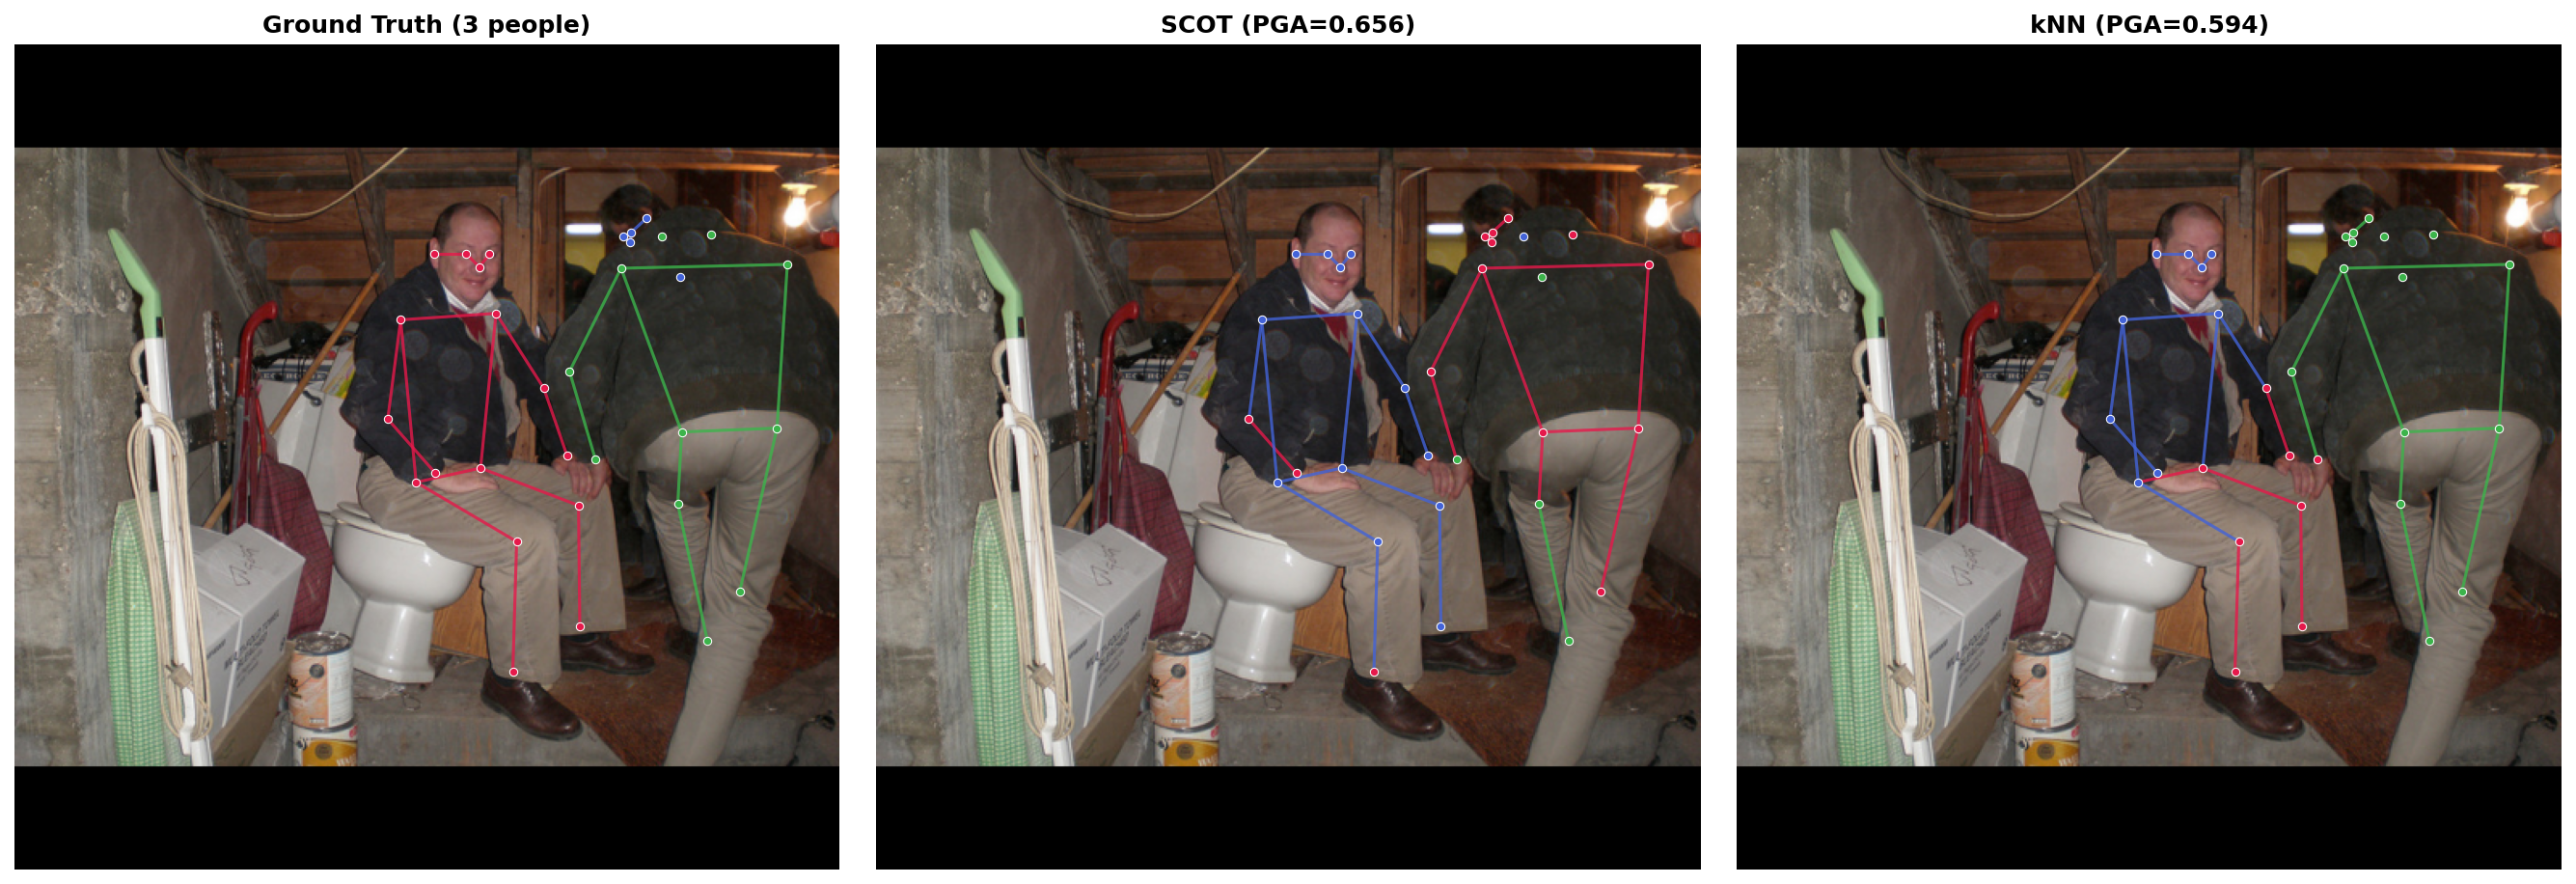
\includegraphics[width=0.85\linewidth]{figures/demo_example_1.png}
    % TODO(figure): replace with a 2x2 grid of representative synthetic
    %               scenes at K=2, K=3, K=4, K=5, with the 17 joint
    %               keypoints overlaid as coloured dots per person and
    %               the skeleton edges drawn as connecting lines.
    %               Goal: show the visual diversity of the synthetic
    %               distribution and the kind of multi-person overlap
    %               that the grouping stage must resolve.
    \caption{Representative scenes from the synthetic dataset
    at person counts $K \in \{2, 3, 4, 5\}$.
    Each panel shows the rendered Blender frame
    with the 17 per-person ground-truth keypoints overlaid
    and colour-coded by person identity.
    The synthetic generator controls camera pose, lighting,
    person placement, and visibility,
    and emits exact metric depth at each joint via raycast,
    which the depth-removal analysis of Section~\ref{sec_meth_data_depth} subsequently discards.}
    \label{fig:synth_examples}
\end{figure}

\subsection{COCO adapter}
\label{sec_meth_data_coco}

For evaluation on real images, the COCO 2017 person-keypoint annotations~\cite{lin2014coco} are loaded via the pycocotools API
and filtered to images containing at least one person.
The native COCO visibility flags ($0 = $ not labelled, $1 = $ occluded, $2 = $ visible) are mapped to the same three-value semantics as the synthetic generator.
COCO does not provide a depth channel,
so the adapter estimates one via MiDaS~\cite{ranftl2020midas},
a pre-trained monocular depth estimator that produces a per-pixel relative depth map from a single RGB image.
The DPT-Hybrid variant is used because it combines convolutional and transformer backbones and is the strongest publicly available checkpoint at moderate inference cost;
the model is instantiated once at adapter construction time
and the depth value at each labelled keypoint pixel is sampled into the $z$ slot of the keypoint vector.
This produces a $[x, y, z, v]$ representation that is dimensionally identical to the synthetic format
and that the downstream pipeline cannot distinguish from synthetic data.

The decision to estimate depth via MiDaS rather than to drop the depth channel for COCO was made
to keep the network architecture identical across data sources.
Section~\ref{sec_meth_data_depth} below describes the subsequent measurement that led to depth being removed for every method in this chapter.

\subsection{Unified pipeline}
\label{sec_meth_data_pipeline}

Both adapters emit the same per-image record:
the image tensor at $[3, H, W]$,
a list of per-person keypoint tensors at $[17, 4]$,
an image identifier,
and the person count.
A single \texttt{PoseDataset} sits behind both adapters and applies a common transform:
each image is resized to fit within $\texttt{target\_size} \times \texttt{target\_size}$ preserving aspect ratio,
symmetrically padded to the exact target dimension,
and the keypoint coordinates are scaled and shifted to match;
the $z$ and $v$ columns are passed through unchanged
and joints with $v = 0$ are not transformed at all.
A custom collate function in the dataloader stacks the image tensors but keeps the per-image keypoint lists as a list-of-lists,
because the per-image person count is variable and PyTorch's default collate cannot batch variable-length structures.

The preprocessor converts each batch into PyTorch Geometric graphs~\cite{fey2019pyg}, one graph per image.
Joints with $v = 0$ are excluded entirely from the graph rather than represented as zero-feature nodes,
so that the message passing has no spurious nodes to aggregate over.
Each surviving joint becomes a node with raw feature vector
\begin{equation}
    \mathbf{x}_i
    = [\,x_{\text{norm}},\; y_{\text{norm}},\; z_{\text{norm}},\; v_{\text{norm}}\,]
    \in \mathbb{R}^{4},
    \label{eq:node_feature_with_depth}
\end{equation}
where the spatial coordinates are normalised to $[0, 1]$ by the image dimensions,
$z_{\text{norm}}$ is a per-graph min-max normalisation of the depth over valid joints,
and $v_{\text{norm}}$ maps the three visibility levels to $\{0.0, 0.5, 1.0\}$.
The per-graph depth normalisation is what makes MiDaS-estimated COCO depth and Blender-rendered synthetic depth dimensionally compatible:
both sources land in $[0, 1]$ regardless of absolute scale.
The vector $\mathbf{x}_i$ is the raw \emph{preprocessed} feature used by the rest of the chapter;
the GAT layer-zero input $\mathbf{h}_i^{(0)}$ of Equation~\eqref{eq:layer0_input} concatenates $\mathbf{x}_i$ with the joint-type embedding.
Separate tensors per graph hold the joint-type indices (consumed by the type embedding)
and the ground-truth person labels (consumed by the contrastive loss at training time).
Edges are built by $k$-nearest neighbours in $(x_{\text{norm}}, y_{\text{norm}}, z_{\text{norm}})$ space with $k = 8$,
chosen as described in Section~\ref{sec_meth_problem_graph}.

\subsection{Removing the depth channel}
\label{sec_meth_data_depth}

The depth channel was removed from every method reported in the headline evaluations,
on the basis of a single diagnostic experiment whose result is reported in Chapter~\ref{chap_4}.
The methodological motivation is recorded here so that the rest of the chapter can refer back to it.

With depth, $k$NN clustering on contrastive GAT embeddings reaches a synthetic-test PGA of $0.994$;
the problem is effectively solved by spatial proximity in three dimensions.
The metric depth produced by the Blender renderer is exact ground truth,
so two people standing at different camera distances are separated by the $z$ coordinate alone,
and the GAT has very little discriminative work to do.
This artificially inflated all synthetic baselines and left no room for the learned heads or for SA-DMoN to demonstrate added value:
any small improvement on a near-perfect baseline is statistically indistinguishable from noise.

On COCO, the depth signal comes from MiDaS rather than from ground truth.
MiDaS produces a \emph{relative} depth ordering with no metric scale,
and the per-image scale varies with the image content.
The synthetic-to-COCO domain gap is therefore amplified by the $z$ channel:
a synthetic model trained on metric depth has learned to read $z$ at a scale that does not exist in the MiDaS output.
Removing depth removes this domain-gap component
and forces every method in this chapter to operate on the same two-dimensional signal that a real bottom-up pipeline has access to without an external depth estimator.

The removal is implemented via a \texttt{use\_depth} flag in the preprocessor configuration.
When the flag is off,
the raw feature vector of Equation~\eqref{eq:node_feature_with_depth} reduces to
\begin{equation}
    \mathbf{x}_i
    = [\,x_{\text{norm}},\; y_{\text{norm}},\; v_{\text{norm}}\,]
    \in \mathbb{R}^{3},
    \label{eq:node_feature_no_depth}
\end{equation}
the $k$NN graph is built on $(x_{\text{norm}}, y_{\text{norm}})$ only,
and the input dimension of the GAT first layer is reduced accordingly via Equation~\eqref{eq:layer0_input}.
Every result reported in Chapter~\ref{chap_4} from the baseline kNN onward uses this no-depth configuration,
unless the row is explicitly labelled as a depth-on diagnostic.

\section{Baseline: Standard GAT with Contrastive Loss}
\label{sec_meth_baseline}

The baseline used for all later comparisons is a standard graph attention network
trained on the synthetic dataset using a contrastive loss -
at inference, the output embeddings are L2-normalised and grouped using $k$-means.
This gives a relatively simple starting point
and sets the bar that any change to the embedding network or grouping method must clear.

The baseline also fixes the main training and evaluation procedure used throughout the experiments -
unless stated otherwise,
later methods inherit the same optimiser, training schedule, and clustering protocol.
This keeps the comparisons consistent
and means that improvements can be linked more directly
to the architectural or methodological change being tested,
rather than to changes in the surrounding training setup.

\subsection{Architecture}
\label{sec_meth_baseline_arch}

The baseline network takes the graph $\mathcal{G}$ constructed in Section~\ref{sec_meth_problem_graph}
and produces an embedding $\mathbf{z}_i \in \mathbb{R}^{d}$ for each node, with $d=128$.
The input to the first GAT layer is the representation $\mathbf{h}_i^{(0)}$
defined in Equation~\eqref{eq:layer0_input} -
in the default no-depth configuration,
this combines the three preprocessed features $\mathbf{x}_i \in \mathbb{R}^{3}$
from Equation~\eqref{eq:node_feature_no_depth}
with a learned 32-dimensional joint-type embedding.
The resulting input dimension is therefore $d_0=35$ -
for the earlier depth-enabled diagnostic,
the four features of Equation~\eqref{eq:node_feature_with_depth} give $d_0=36$.

Message passing is performed by two GATv2 layers~\cite{brody2022gatv2},
each using four attention heads and a hidden dimension of 64.
GATv2 is used instead of the original GAT~\cite{velickovic2018gat}
because its attention mechanism allows the ranking of neighbouring nodes to depend on the query node -
as discussed in Section~\ref{sec_meth_gat},
the original GAT is limited by its static attention formulation,
while GATv2 changes the order of the linear projection and nonlinearity
to produce dynamic attention~\cite{brody2022gatv2}.

This distinction is useful for pose grouping
because not every neighbour should contribute in the same way -
a keypoint may need to treat a nearby joint of the same type
differently from an anatomically related joint of another type.
The importance of a neighbour therefore depends on both nodes involved in the interaction -
for this reason,
GATv2 is kept as the attention primitive throughout the methods developed in this chapter.

After the two message-passing layers,
a linear projection maps each node representation to the 128-dimensional embedding space -
the output is then L2-normalised,
placing each embedding on the unit hypersphere $\mathbb{S}^{d-1}$.
This matches the cosine-based contrastive objective used during training
and also gives the downstream $k$-means stage a bounded representation space.
The complete baseline architecture is summarised in Table~\ref{tab:baseline_arch}.

\begin{table}[H]
\centering
\footnotesize
\begin{tabular}{ll}
\toprule
Component & Setting \\
\midrule
Attention primitive            & GATv2~\cite{brody2022gatv2} \\
Number of GAT layers           & 2 \\
Number of attention heads      & 4 \\
Hidden dimension               & 64 \\
Output (embedding) dimension   & 128 \\
Joint-type embedding dimension & 32 \\
Layer normalisation            & yes \\
Output normalisation           & L2 (unit hypersphere) \\
Dropout                        & 0.1 \\
\bottomrule
\end{tabular}
\caption{Baseline GAT architecture used as the comparison point for the
methods evaluated in this chapter - methods inherit these settings
unless a parameter is explicitly changed or included in a later sweep.
The architecture sweep used to select the final PG-GAT configuration
is described in Section~\ref{sec_meth_pggat_training}.}
\label{tab:baseline_arch}
\end{table}

\subsection{Contrastive loss}
\label{sec_meth_baseline_loss}

The embedding network is trained using a margin-based contrastive loss~\cite{chopra2005contrastive}
defined on cosine similarity.
For a graph containing $N$ keypoints
with ground-truth person labels $\mathbf{y}^\star \in \{1,\dots,K\}^{N}$,
the cosine similarity between two L2-normalised embeddings is
\begin{equation}
    \cos(\mathbf{z}_i,\mathbf{z}_j)
    = \mathbf{z}_i^\top \mathbf{z}_j.
\end{equation}
Training pairs are divided into two sets -
positive pairs contain keypoints belonging to the same person,
\begin{equation}
    \mathcal{P}^{+}
    = \{(i,j) :
    \mathbf{y}^\star_i = \mathbf{y}^\star_j,\; i \neq j\},
\end{equation}
while negative pairs contain keypoints belonging to different people,
\begin{equation}
    \mathcal{P}^{-}
    = \{(i,j) :
    \mathbf{y}^\star_i \neq \mathbf{y}^\star_j\}.
\end{equation}
The contrastive objective is then
\begin{equation}
    \mathcal{L}_{\text{contrastive}}
    =
    \frac{1}{|\mathcal{P}^{+}|}
    \sum_{(i,j) \in \mathcal{P}^{+}}
    \bigl(
        1 - \cos(\mathbf{z}_i,\mathbf{z}_j)
    \bigr)
    \;+\;
    \frac{1}{|\mathcal{P}^{-}|}
    \sum_{(i,j) \in \mathcal{P}^{-}}
    \max\!\bigl(
        0,\;
        \cos(\mathbf{z}_i,\mathbf{z}_j) - \gamma
    \bigr).
    \label{eq:contrastive_loss}
\end{equation}
The first term pulls embeddings belonging to the same person towards a cosine similarity of 1 -
positive pairs keep contributing to the loss however close they already are.
The second term penalises different-person pairs whose similarity exceeds the margin $\gamma$ -
once a negative pair has been pushed below $\gamma$ it no longer contributes,
which keeps the gradient focused on the negative pairs that are still too close together.

The margin is set to $\gamma=0.5$ for the experiments in this work -
this value is later tested as part of the 24-run Bayesian loss sweep
described in Section~\ref{sec_meth_pggat_training},
which confirms it as near-optimal.
The same contrastive formulation is kept across the main embedding experiments,
allowing changes in performance to be attributed more directly to the network architecture
rather than to a different training objective.

The symbol $\gamma$ is used for the contrastive margin throughout this chapter -
this avoids confusion with $m$,
which is already used in Section~\ref{sec_meth_dmon_prelim} to denote the total number of graph edges.

\subsection{Training schedule and grouping read-out}
\label{sec_meth_baseline_training}

The baseline model is trained for 50 epochs
using the 400-scene synthetic training split with a batch size of 4.
Optimisation uses AdamW~\cite{loshchilov2019adamw}
with an initial learning rate of $10^{-3}$ and weight decay of $10^{-4}$ -
a cosine-annealing schedule~\cite{loshchilov2017cosineannealing}
reduces the learning rate to $10^{-5}$ over the course of training.
Gradient norms are clipped at $1.0$ to reduce the effect of occasional large updates,
particularly from batches containing more densely populated scenes.

The model is evaluated every five epochs
on the 100-scene synthetic validation split
using the PGA metric defined in Equation~\eqref{eq:pga} -
rather than using the final training epoch automatically,
the checkpoint with the highest validation PGA is kept for evaluation.

At inference,
the trained network is applied once to each image
to produce the set of node embeddings $\{\mathbf{z}_i\}_{i=1}^{N}$ -
these embeddings are already L2-normalised and are grouped using $k$-means with $k=K$.
The scikit-learn implementation~\cite{scikitlearn} is used
with ten random initialisations and a fixed random seed -
the resulting cluster labels are matched to the ground-truth person labels
using the Hungarian assignment,
after which PGA is calculated using Equation~\eqref{eq:pga}.

Chapter~\ref{chap_4} reports two versions of this baseline -
the first is the depth-enabled configuration
using the four-dimensional node features of Equation~\eqref{eq:node_feature_with_depth}.
This is kept as a diagnostic result because,
as discussed in Section~\ref{sec_meth_data_depth},
exact synthetic depth makes the grouping task unusually easy -
the second is the no-depth configuration using Equation~\eqref{eq:node_feature_no_depth}.
This becomes the main baseline for the experiments that follow.

Unless stated otherwise,
the methods from Section~\ref{sec_meth_learned_heads} onward inherit this no-depth setting
together with the 50-epoch training schedule and optimiser configuration described above -
the architecture settings in Table~\ref{tab:baseline_arch}
are the manually selected baseline values used by the learned-head and SA-DMoN experiments.

PG-GAT later performs a separate Bayesian architecture search,
described in Section~\ref{sec_meth_pggat_training},
which selects a larger three-layer network with a 256-dimensional output -
the two-layer baseline is therefore the bar
that any modification of the embedding network or grouping head must clear at matched compute,
rather than the final architecture used by PG-GAT.
\section{Learned Grouping Heads}
\label{sec_meth_learned_heads}

Three learned grouping heads are constructed on top of the baseline GAT embedding network of Section~\ref{sec_meth_baseline}.
Each is a different attempt to push the grouping decision into a learnable component
rather than reading off the structure of the embedding space with $k$-means.
The mathematical preliminaries for each head are given in Section~\ref{sec_meth_clustering};
this section describes how each was adapted to the pose-grouping problem,
the loss it minimises during joint training with the GAT,
and the read-out used at inference.
None of the three improves on plain $k$-means in the headline evaluations of Chapter~\ref{chap_4},
and the resulting evidence motivates the shift of attention to the embedding network itself in Section~\ref{sec_meth_pggat}.

\subsection{Deep embedded clustering on pose embeddings}
\label{sec_meth_dec_pose}

The DEC head~\cite{xie2016dec} treats grouping as a fully unsupervised problem on top of the GAT embeddings.
At training time the head maintains $K$ cluster centres $\boldsymbol{\mu}_1, \dots, \boldsymbol{\mu}_K \in \mathbb{R}^{d}$
in the same embedding space as the GAT output.
At each forward pass over a scene with $K$ ground-truth people,
the centres are initialised by $k$-means++~\cite{arthur2007kmeanspp} on the current GAT embeddings of that scene;
this per-scene initialisation is the methodological adaptation that makes DEC applicable to a setting where every image has a different $K$
rather than a fixed cluster count over a single dataset.

Given embeddings $\{\mathbf{z}_i\}$ and centres $\{\boldsymbol{\mu}_k\}$,
the soft assignment under a Student's $t$-distribution with one degree of freedom~\cite{vandermaaten2008tsne} is
\begin{equation}
    q_{ik}
    = \frac{\bigl(1 + \|\mathbf{z}_i - \boldsymbol{\mu}_k\|_2^2\bigr)^{-1}}
           {\sum_{k'} \bigl(1 + \|\mathbf{z}_i - \boldsymbol{\mu}_{k'}\|_2^2\bigr)^{-1}},
    \label{eq:dec_q}
\end{equation}
and the sharpened target distribution is
\begin{equation}
    p_{ik}
    = \frac{q_{ik}^2 / f_k}{\sum_{k'} q_{ik'}^2 / f_{k'}},
    \quad f_k = \sum_i q_{ik}.
    \label{eq:dec_p}
\end{equation}
The loss is the Kullback--Leibler divergence between target and prediction,
$\mathcal{L}_{\text{DEC}} = \sum_{i,k} p_{ik} \log (p_{ik} / q_{ik})$,
combined additively with the contrastive loss of Equation~\eqref{eq:contrastive_loss}.
The target $\mathbf{p}$ is computed with \texttt{torch.no\_grad} and treated as a fixed target
so the gradient flows only through $\mathbf{q}$:
the head learns to make its soft assignments more confident over time,
and the underlying GAT receives gradient signal through the dependence of $\mathbf{q}$ on the embeddings.

DEC is the only head in this section that does not consume ground-truth person labels in its own loss.
The contrastive loss still uses the labels, so the GAT receives supervised signal;
the DEC head itself is unsupervised
and the methodological prediction from this asymmetry --- the head can only sharpen assignments that are already roughly correct, it has no signal to fix wrong ones ---
is corroborated by the result in Section~\ref{sec_results_learned_heads}.

\subsection{Slot attention on pose embeddings}
\label{sec_meth_slot_pose}

The slot attention head~\cite{locatello2020slotattention} is supervised by the ground-truth person labels via Hungarian-matched cross entropy.
$K$ slot vectors $\mathbf{s}_1, \dots, \mathbf{s}_K \in \mathbb{R}^{d}$ are initialised independently for each scene
by sampling from a learned Gaussian distribution $\mathcal{N}(\boldsymbol{\mu}, \boldsymbol{\sigma}^2 \mathbf{I})$
whose parameters are trained jointly with the GAT.
The slots then iteratively refine themselves
via a competitive attention mechanism over the GAT embeddings.
At each iteration $t$,
queries are obtained by layer-normalising the slots,
keys and values are obtained by layer-normalising the embeddings,
and an attention matrix is computed by softmax \emph{across slots} (rather than the standard softmax across keys),
which enforces competition between slots for each joint.
The matrix is then row-normalised and used to weight the values into per-slot updates,
which a GRU cell~\cite{cho2014gru} mixes into the previous slot state,
followed by a residual feed-forward block.
After $T = 7$ iterations the final slots produce logits $\ell_{ik} = \mathbf{z}_i^\top \mathbf{W}_{\text{key}} \mathbf{s}_k$
for each joint--slot pair.

The training loss is Hungarian-matched cross entropy:
the optimal cluster-to-person bijection $\pi^\star$ is computed by Hungarian assignment on the per-slot mean prediction probability against each ground-truth person,
and the cross-entropy loss is computed against the permuted ground-truth labels $\pi^\star \circ \mathbf{y}^\star$.
At inference the slots are run identically and the argmax of the logits gives the partition.
Iteration count and learning-rate schedule are fixed by the values that stabilised the isolation tests recorded earlier in this chapter:
seven iterations rather than the standard three,
and a cosine schedule decaying from $10^{-3}$ to $10^{-5}$
to avoid the overshoot that a constant learning rate produced at three iterations.

\subsection{Graph partitioning on pose embeddings}
\label{sec_meth_partition_pose}

The graph partitioning head reframes grouping as binary edge classification on the keypoint graph,
rather than as an explicit partition into $K$ clusters.
A pair MLP $\phi_{\text{pair}} : \mathbb{R}^{2d} \to \mathbb{R}$ predicts,
for every pair of joints $(i, j)$ in the graph,
the logit of the event ``$i$ and $j$ belong to the same person''.
The input to the MLP is the concatenation of the embedding difference and the embedding element-wise product:
\begin{equation}
    \phi_{\text{pair}}\!\bigl([\,\mathbf{z}_i - \mathbf{z}_j \,\big\|\, \mathbf{z}_i \odot \mathbf{z}_j\,]\bigr)
    \in \mathbb{R}.
    \label{eq:partition_pair}
\end{equation}
This is the standard pair-feature construction from face-clustering GNN literature~\cite{yang2020gcnve}:
the difference encodes direction in embedding space and the product encodes co-activation magnitude.

The loss is binary cross entropy over all $\binom{N}{2}$ pairs.
Positive pairs (same person) are far less numerous than negative pairs;
for the synthetic scenes with five people and seventeen joints,
the ratio is approximately $680$ positives to $2890$ negatives.
The positive class is up-weighted by $\texttt{pos\_weight} = \min(10, n_{\text{neg}} / n_{\text{pos}})$
to prevent the loss being dominated by negative pairs.
At inference the predicted affinities are thresholded at $0.5$
and connected components on the resulting binary affinity graph are recovered by union--find.

Graph partitioning is the only head of the three for which $K$ is not required at inference:
the number of connected components is read directly from the predicted affinities,
which makes the head structurally appealing for the autonomous-pipeline use case of Section~\ref{sec_meth_integration}.
The Chapter~\ref{chap_4} results explain why this structural advantage does not translate into a competitive transfer result.

\subsection{Joint training schedule}
\label{sec_meth_learned_heads_training}

All three heads are trained jointly with the GAT for 50 epochs on the synthetic training split
using the optimiser settings of Section~\ref{sec_meth_baseline_training}.
The total loss is the sum of the contrastive loss of Equation~\eqref{eq:contrastive_loss}
and the head-specific loss with a head weight set to $1.0$;
this configuration was retained from the initial isolation tests for each head
on the basis that none of the heads benefited from a sweep over the head weight in early experiments,
and any deeper sweep would have run against the resource budget allocated to the eventually successful PG-GAT investigation.
Validation, checkpointing, and the PGA read-out follow the conventions of Section~\ref{sec_meth_baseline_training};
the head's own forward pass is used at inference for DEC and slot attention,
while the partition head's connected components are read directly as the final assignment.

\section{SA-DMoN --- Skeleton-Aware Deep Modularity Networks}
\label{sec_meth_sadmon}

The three learned grouping heads from
Section~\ref{sec_meth_learned_heads} all fail to improve on plain
$k$-means when applied to embeddings from the same GAT backbone.
This section considers a different approach.
The GAT backbone is retained -
but the grouping stage is replaced with a Deep Modularity Network
(DMoN)~\cite{tsitsulin2023dmon},
where the training objective is based on a differentiable relaxation
of Newman modularity~\cite{newman2006modularity}.

A vanilla DMoN configuration is tested first,
followed by nine skeleton-aware variants
that modify different parts of the modularity formulation.
Despite these changes, all ten configurations
plateau within a relatively narrow performance range
and remain below the $k$-means baseline.
The experiments point to a structural problem
with the modularity objective in this setting -
its null model is misaligned with a graph
whose edges are constructed from spatial proximity
between keypoints.

Together with the learned-head experiments of
Section~\ref{sec_meth_learned_heads},
these results provide further evidence
that changing the grouping head is not the main source of improvement.
Instead, the quality of the embedding produced by the network
is the binding constraint.

\subsection{Vanilla DMoN}
\label{sec_meth_dmon_pose}

Given the keypoint graph $\mathcal{G}$ from
Section~\ref{sec_meth_problem_graph} - with adjacency matrix
$A \in \{0,1\}^{N \times N}$ -
DMoN predicts a soft cluster-assignment matrix
$\mathbf{S} \in [0,1]^{N \times K}$.
Each row of $\mathbf{S}$ sums to one,
so that $S_{ik}$ represents the soft assignment
of node $i$ to cluster $k$.
The assignments are produced by applying a single linear projection
to the GAT embeddings followed by a softmax over the $K$ clusters.

The standard DMoN objective contains three
terms~\cite{tsitsulin2023dmon}:
\begin{equation}
    \mathcal{L}_{\text{DMoN}}
    = -\frac{1}{2m}\mathrm{Tr}\bigl(\mathbf{S}^\top \mathbf{B}\,\mathbf{S}\bigr)
      + \lambda_{\text{ortho}}\,
      \Bigl\|\mathbf{S}^\top \mathbf{S}/\|\mathbf{S}^\top \mathbf{S}\|_F - \mathbf{I}/\sqrt{K}\Bigr\|_F
      + \lambda_{\text{cluster}}\,\Bigl(\tfrac{\sqrt{K}}{N}\,\|\mathbf{s}_{\text{vol}}\|_2 - 1\Bigr),
    \label{eq:dmon_loss}
\end{equation}
where
\begin{equation}
    \mathbf{B}
    =
    \mathbf{A}
    -
    \frac{\mathbf{d}\mathbf{d}^{\top}}{2m}
\end{equation}
is the modularity matrix,
$\mathbf{d}$ contains the node degrees,
and $m = \tfrac{1}{2}\sum_{ij} A_{ij}$ is the total number of edges.
The first term encourages partitions with high modularity.
The orthogonality term discourages highly unbalanced assignments,
while the term weighted by $\lambda_{\text{cluster}}$
helps prevent solutions in which one or more clusters collapse
and receive no nodes.

Two further terms are added to the DMoN objective.
The first is a supervised cross-entropy term,
computed against the ground-truth person labels $\mathbf{y}^\star$
after Hungarian matching of clusters to people,
with weight $\lambda_{\text{supervised}}=1$.
This keeps the predicted clusters aligned with person identity,
rather than allowing the network to follow only the partition
preferred by the modularity objective.
The second is a type-exclusivity term with weight $\lambda_{\text{type}}=1$,
which penalises a cluster that accumulates
more than one joint of the same type.
In the implementation,
the spectral term itself also carries a weight,
with $\lambda_{\text{spectral}}=0.1$ unless a configuration below changes it.

This vanilla configuration forms the starting point
for the SA-DMoN experiments reported in Chapter~\ref{chap_4}.
Its main limitation comes from the structure of the graph itself.
Modularity rewards groups of nodes
that are more densely connected than expected under its null model,
while the keypoint graph is constructed from spatial proximity.
As a result, nearby joints are encouraged to remain together
even when they belong to different people.
Pose grouping often requires exactly the opposite behaviour.
This mismatch motivates the skeleton-aware modifications
to the null model introduced in the next subsection.

\subsection{SA-DMoN v1: a skeleton-aware null model}
\label{sec_meth_sadmon_v1}

The v1 variant replaces the standard degree-based null model
$\mathbf{N}_{\text{deg}} = \mathbf{d}\mathbf{d}^\top/(2m)$ with one
that includes both spatial proximity and the known structure of the
COCO skeleton.
The spatial component is defined using a Gaussian kernel
over the normalised keypoint positions
\begin{equation}
    P_{ij}
    =
    \exp\!\Bigl(
        -\,\frac{\|\mathbf{p}_i-\mathbf{p}_j\|_2^2}{2\sigma^2}
    \Bigr),
    \label{eq:sadmon_spatial}
\end{equation}
where $\sigma$ controls the spatial bandwidth
and is treated as a hyperparameter below.

The skeleton component is represented by a fixed $17 \times 17$
joint-type affinity matrix $T$,
constructed using breadth-first search over the COCO skeleton graph.
Joint types that are directly connected in the skeleton
are assigned an affinity of $T_{ab}=1.0$.
Pairs separated by two hops receive $0.5$,
and three-hop pairs receive $0.25$.
Joint types more than three hops apart -
or otherwise topologically disconnected -
receive an affinity of zero.

For nodes $i$ and $j$ with joint types $a$ and $b$, respectively,
the spatial and skeleton terms are combined as
\begin{equation}
    R_{ij}
    =
    T_{ab} \cdot P_{ij}.
    \label{eq:sadmon_null}
\end{equation}
The resulting matrix is rescaled so that its total mass matches the
edge mass of the original graph,
\begin{equation}
    \tilde{R}_{ij}
    =
    R_{ij}
    \left(
        \frac{2m}{\sum_{ij}R_{ij}}
    \right).
\end{equation}
The pose-specific modularity matrix is then
\begin{equation}
    \mathbf{B}_{\text{pose}}
    =
    \mathbf{A} - \tilde{\mathbf{R}},
\end{equation}
which replaces $\mathbf{B}$ in the DMoN loss of
Equation~\eqref{eq:dmon_loss}.
The remaining parts of the model are left unchanged,
including the assignment head,
the orthogonality and collapse-prevention terms,
and the supervised cross-entropy and type-exclusivity terms.

The bandwidth $\sigma$ proved to be the main sensitive parameter in
this formulation.
Several versions were therefore tested to determine
whether the behaviour of the null model was mainly caused by how this
bandwidth was selected.
Each configuration below corresponds to one of
the SA-DMoN ablations reported in Chapter~\ref{chap_4}.

\begin{compactenum}
    \item \textbf{Learnable, unconstrained.}
        The bandwidth is parameterised as $\sigma=\exp(\xi)$,
        with $\xi$ initialised to $\log 0.2$,
        and optimised with the rest of the network.
        This allows the model to choose its own spatial
        scale.

    \item \textbf{Learnable, clamped.}
        The same learnable parameterisation is used -
        but $\sigma$ is clamped to the range $[0.05,0.5]$
        during the forward pass.
        This prevents the bandwidth from diverging,
        as observed in the unconstrained configuration.

    \item \textbf{Learnable, clamped, $\lambda_{\text{spectral}}=1$.}
        This uses the clamped bandwidth while increasing the weight of
        the spectral term so that it has the same weighting as the
        supervised loss.
        The purpose is to test whether the modularity
        signal becomes useful when it has a larger influence on
        training.

    \item \textbf{Fixed at the per-graph median pairwise distance.}
        Here, $\sigma$ is recalculated for each scene as the median
        pairwise keypoint distance using \texttt{torch.no\_grad}.
        This gives a bandwidth that adapts to the spatial scale
        of the scene without allowing the optimiser to change it directly.

    \item \textbf{Spectral term removed.}
        The spectral weight is set to $\lambda_{\text{spectral}}=0$.
        The skeleton-aware null model is still calculated
        for diagnostic purposes -
        but it contributes no modularity gradient during training.
        This configuration separates the effect of the supervised loss
        from the modularity-based objective.
\end{compactenum}

These five v1 configurations form the methodological basis
of SA-DMoN Experiments~4--8 reported in Chapter~\ref{chap_4}.

\subsection{SA-DMoN v2: decoupled adjacency and entropy type loss}
\label{sec_meth_sadmon_v2}

The motivation for the v2 variants comes from a limitation observed in
the v1 formulation.
The spatial adjacency $\mathbf{A}$ and the spatial
component of the null model $\mathbf{P}$ are both strongly determined
by keypoint distance.
As a result, the two terms in
$\mathbf{B}_{\text{pose}} = \mathbf{A} - \tilde{\mathbf{R}}$ can
partially cancel around the selected bandwidth,
weakening the modularity signal available during training.

The v2 formulation tests two changes intended to address this problem.
The first separates the adjacency used by the modularity loss
from the geometric graph used for message passing.
The second replaces the threshold-based type-exclusivity loss
used in v1 with a smoother entropy-based objective.
The two changes are independent and can also be used together,
giving four configurations in total.

\textbf{Fix~1: feature-based adjacency:}
Instead of using the geometric $k$NN adjacency from
Section~\ref{sec_meth_problem_graph} inside the spectral loss,
a new adjacency is constructed from the current GAT embeddings.
This feature graph is formed using $k$-nearest neighbours
in embedding space with $k=8$.
The original geometric graph is still used by the GAT
for message passing -
only the adjacency supplied to the modularity objective is changed.
Since the embedding itself changes during training,
the feature-based graph is reconstructed on each forward pass.

This separates the two roles played by the graph.
Message passing still uses spatial proximity to define
which keypoints exchange information,
while the modularity objective operates on neighbourhoods
learned in the embedding space,
rather than another distance-based version of the same spatial graph.

\textbf{Fix~2: entropy type loss:}
The second change replaces the v1 type-exclusivity term
with a soft entropy-based objective
\begin{equation}
    \mathcal{L}_{\text{type}}^{\text{v2}}
    =
    -\sum_{i,k}
    S_{ik}\,\log p^{\text{type}}_{ik},
\end{equation}
where $p^{\text{type}}_{ik}$ is the estimated probability
that cluster $k$ contains the joint type $t_i$,
calculated from the current soft assignment statistics.
Compared with the threshold-based ReLU formulation used in v1,
this gives a smoother gradient as the assignments change.
The trade-off is that the sharper discrete hinge
of the earlier loss is no longer present.

\textbf{Configurations:}
Four v2 configurations are evaluated in Chapter~\ref{chap_4}.
The first uses feature-based adjacency with
$\lambda_{\text{spectral}}=1.0$.
The second uses the same feature adjacency
but reduces the spectral weight to
$\lambda_{\text{spectral}}=0.1$ -
matching the weighting used in v1.
The third keeps the original spatial adjacency
and changes only the supervised term to the entropy type loss.
The final configuration combines both changes -
using feature-based adjacency together with the
entropy-based type objective.

\subsection{Training schedule}
\label{sec_meth_sadmon_training}

All ten SA-DMoN variants are trained jointly with the GAT on the
synthetic training split.
These include the vanilla DMoN baseline,
the five v1 configurations described above,
including the no-spectral diagnostic,
and the four v2 configurations.
Training otherwise follows the optimiser settings given in
Section~\ref{sec_meth_baseline_training}.

Depending on the behaviour of the head loss,
each configuration is trained for either 100 or 150 epochs.
A 100-epoch schedule is used when the loss has clearly plateaued
by that point.
For configurations where the head loss is still changing at 100 epochs,
training is extended to 150 epochs
to allow additional time for convergence.
This avoids discarding a variant simply because its grouping objective
converges more slowly than the baseline contrastive model.

Despite the longer training schedules,
none of the SA-DMoN configurations are able to improve
improve on $k$-means applied to the baseline GAT embeddings.
The experimental results are reported in
Section~\ref{sec_res_sadmon}.
The broader reason for this behaviour -
particularly the mismatch between the modularity objective
and the structure of the pose-grouping graph -
is discussed in Section~\ref{sec_disc_modularity_autonomy_gap}.

\section{PG-GAT --- Pose Grouping Graph Attention Network}
\label{sec_meth_pggat}

This section describes the methodological centrepiece of the work:
PG-GAT, a skeleton-aware modification of the baseline GATv2 embedding network of Section~\ref{sec_meth_baseline}.
Three modifications to the attention mechanism are introduced,
each motivated by a specific failure mode of the baseline and each independently configurable for ablation,
and a two-stage training schedule (synthetic pre-training followed by COCO fine-tuning)
that is itself defended by a Bayesian sweep over fine-tune hyperparameters.
Every PG-GAT design choice is justified by reference to a sweep, an ablation, or a prior failure recorded earlier in this chapter.

\subsection{Design intuition}
\label{sec_meth_pggat_intuition}

The motivation for PG-GAT follows directly from the experimental evidence presented in Section~\ref{sec_meth_learned_heads} and Section~\ref{sec_meth_sadmon}.
Three independent learned grouping heads (DEC, slot attention, graph partitioning)
and ten variants of a skeleton-aware modularity objective (SA-DMoN v1 and v2)
all failed to outperform plain $k$-means clustering on the standard GAT embeddings.
The persistent failure of learned heads on the same embedding rules out the grouping head as the binding constraint
and identifies the embedding network as the dominant axis of variation.
PG-GAT acts on the embedding stage alone:
the grouping read-out remains the same $k$-means as in the baseline,
and every modification described below changes how the attention mechanism processes the skeleton graph
rather than introducing a new learned component on top of the embedding.

The standard GATv2 attention function~\cite{brody2022gatv2} is type-agnostic with respect to edges:
the same parameters compute attention coefficients for a left-shoulder--left-elbow edge,
a left-shoulder--right-shoulder edge,
and a left-shoulder--right-ankle edge.
These edges carry categorically different information for pose grouping.
A same-type pair must belong to different people, an edge that connects two skeletally adjacent joints is the strongest evidence of a same-person grouping, and a far-apart cross-body pair carries little signal.
PG-GAT introduces three mechanisms that surface this categorical edge structure to the attention layer
without replacing the GATv2Conv primitive that the baseline relies on.

\begin{figure}[H]
    \centering
    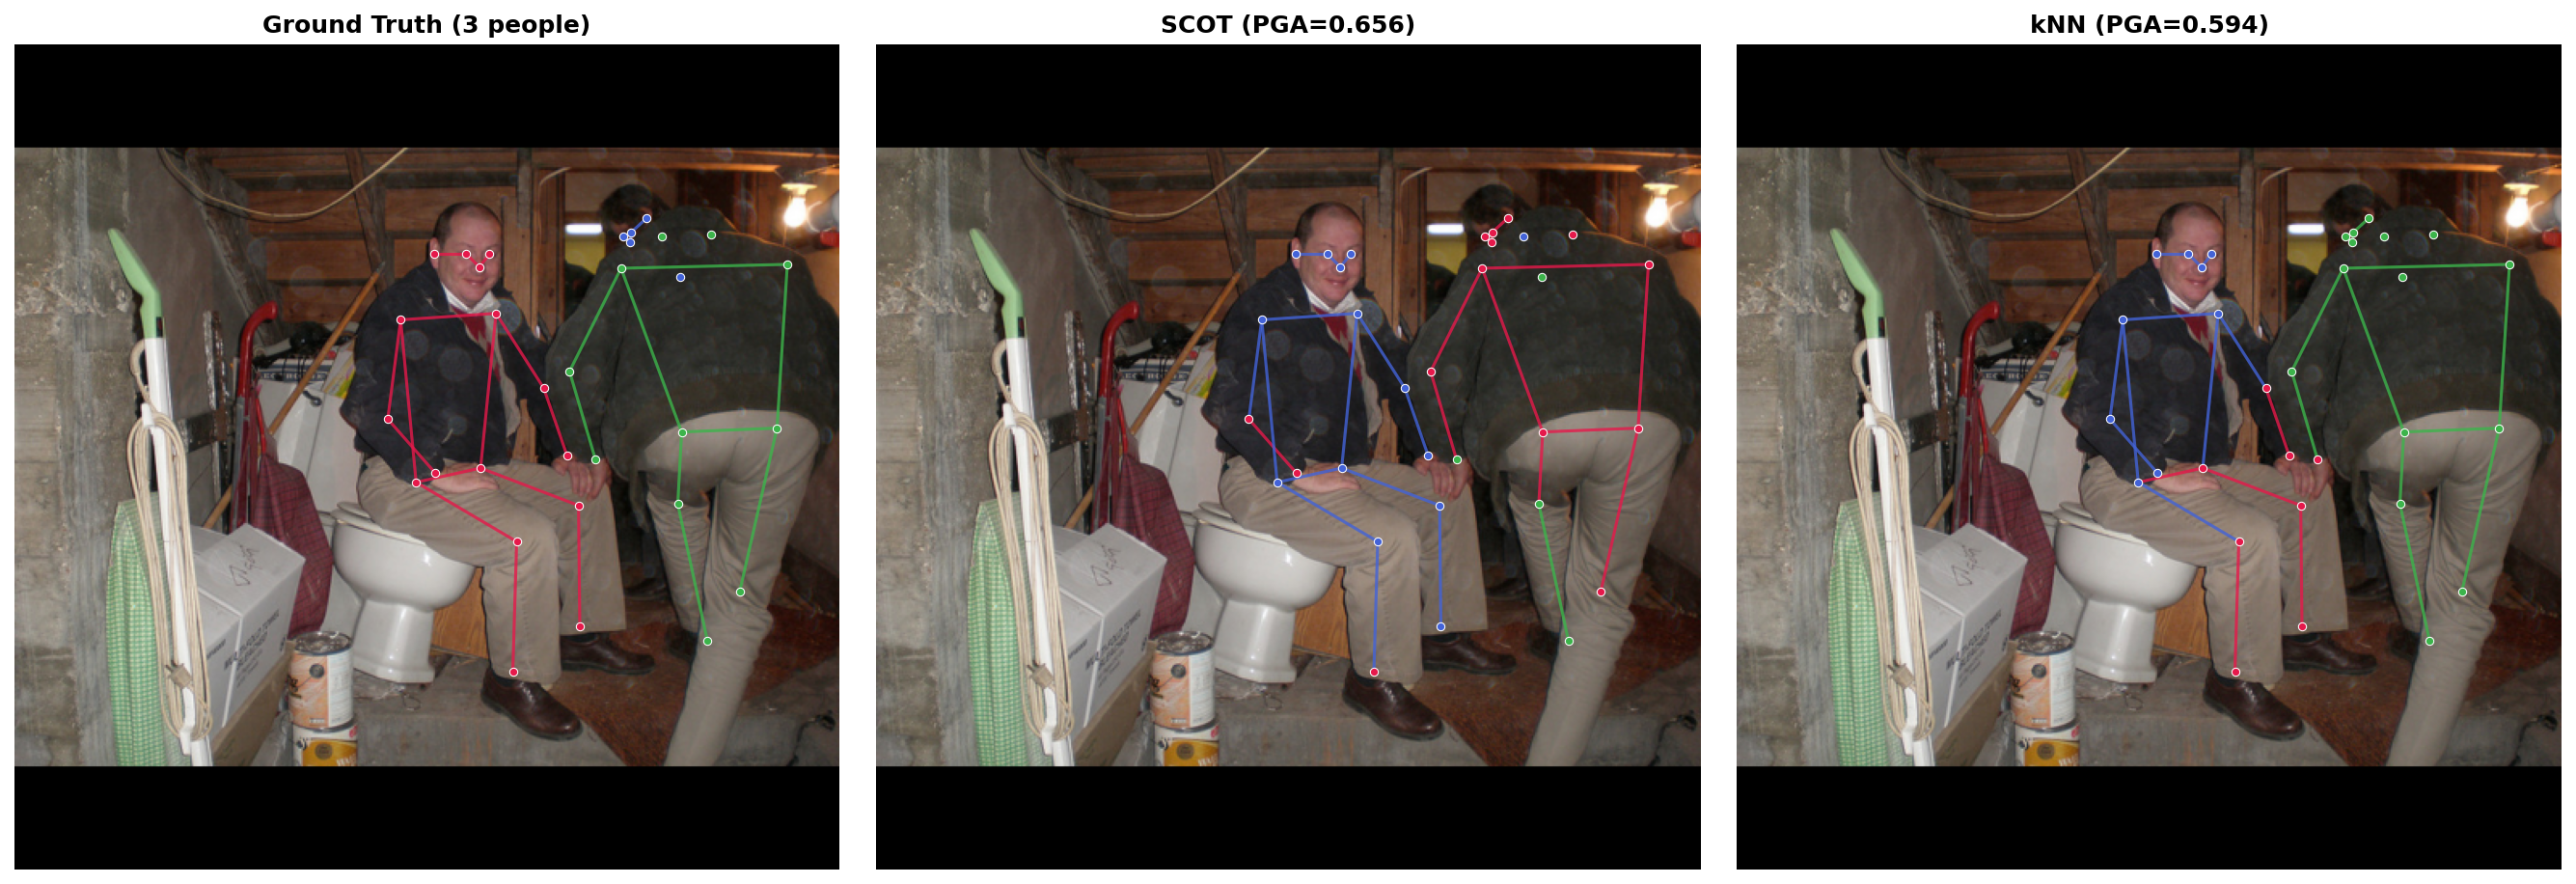
\includegraphics[width=0.9\linewidth]{figures/demo_example_1.png}
    % TODO(figure): replace with a block diagram of PG-GAT showing:
    %   (a) input node features (position, visibility, type embedding)
    %   (b) edge feature constructor producing the 7-dim edge vector
    %       (4-way category one-hot + L2 distance + skeleton hop + same-type flag)
    %   (c) stacked GATv2Conv layers (3 of them per the architecture sweep)
    %       split into a 3-head standard sub-layer and a 1-head repulsion
    %       sub-layer that masks all non-same-type edges
    %   (d) final linear projection + L2 normalisation to embedding dim 256
    % The three colour-highlighted modifications (1: type-pair bias,
    % 2: position encoding, 3: repulsion heads) should be visually
    % distinguishable as the contribution boundaries.
    \caption{The PG-GAT architecture.
    Input node features are the keypoint position, the visibility flag,
    and a learnable joint-type embedding.
    Modification~1 attaches a four-way edge-category one-hot to every edge
    that enters the GATv2 attention as a learned additive bias (red).
    Modification~2 concatenates three geometric edge features
    (L2 distance, skeleton hop distance, same-type indicator)
    onto that one-hot before the same edge encoder (blue).
    Modification~3 splits the multi-head attention into a standard sub-layer
    over the full neighbourhood and a repulsion sub-layer
    whose attention mask restricts it to same-type edges only (green).
    Each modification is independently configurable via a boolean flag,
    which allows the ablation experiments of Chapter~\ref{chap_4} to isolate its marginal contribution.}
    \label{fig:pggat_architecture}
\end{figure}

\subsection{Modification~1: type-pair attention bias}
\label{sec_meth_pggat_typeattn}

Every edge $(i, j) \in \mathcal{E}$ is categorised into one of four mutually exclusive classes based on the joint-type pair $(t_i, t_j)$:
\begin{compactitem}
    \item \textsc{Same-Type} --- $t_i = t_j$, indicating two keypoints that must belong to different people.
        Two left elbows in the same image cannot share an identity.
    \item \textsc{Skeletal-Neighbour} --- $(t_i, t_j)$ is a directly adjacent pair on the COCO skeleton graph (e.g.\ shoulder--elbow).
        The strongest cue for same-person grouping:
        anatomically connected joints from the same person have consistent spatial relationships.
    \item \textsc{Same-Limb} --- $(t_i, t_j)$ lies on the same limb chain but is not directly adjacent (e.g.\ shoulder--wrist).
        Provides medium-range structural information.
    \item \textsc{Cross-Body} --- otherwise.
        Carries weak or no structural prior.
\end{compactitem}
The category is represented as a one-hot vector $\mathbf{c}_{ij} \in \{0,1\}^{4}$
and passed through a small edge-encoder MLP $\phi_{\text{edge}}$ to produce an edge feature
$\mathbf{e}_{ij}^{\text{cat}} = \phi_{\text{edge}}(\mathbf{c}_{ij}) \in \mathbb{R}^{d_e}$.
This edge feature enters the GATv2 attention coefficient via the standard \texttt{edge\_dim} mechanism of PyG's \texttt{GATv2Conv} implementation~\cite{fey2019pyg},
which extends the attention pre-activation by an additive learned edge bias:
\begin{equation}
    \alpha_{ij}^{(l)}
    \propto \exp\!\Bigl(
        \mathbf{a}^{(l)\top}
        \mathrm{LeakyReLU}\!\bigl(
            \mathbf{W}^{(l)} [\,\mathbf{h}_i^{(l)} \,\|\, \mathbf{h}_j^{(l)}\,]
            + \mathbf{W}_e^{(l)} \mathbf{e}_{ij}^{\text{cat}}
        \bigr)
    \Bigr),
    \label{eq:pggat_typeattn}
\end{equation}
where the learnable parameters $\mathbf{a}^{(l)}$, $\mathbf{W}^{(l)}$, and $\mathbf{W}_e^{(l)}$ are GATv2 layer-$l$ weights.
The four edge categories therefore enter the attention as four learnable additive biases that the network can adjust independently
without disturbing the underlying GATv2Conv numerics.

The decision to inject category information as an edge feature rather than as a per-category weight tensor
was made on the basis of an initial implementation that used custom scatter-based attention with per-category projection matrices.
That implementation failed catastrophically (synthetic PGA $0.60$) due to numerical instability in the manual softmax over scattered scores;
switching to GATv2Conv with edge features recovered stable training and removed the instability without affecting expressive power.

\subsection{Modification~2: skeleton-relative position encoding}
\label{sec_meth_pggat_posenc}

The baseline GAT carries no explicit spatial information in its attention coefficients:
positional information is present only as a node feature
and is mixed indiscriminately with the type embedding and visibility.
The second modification injects three geometric edge features
that surface relative-geometry information directly to the attention mechanism:
\begin{compactitem}
    \item the L2 distance between the two endpoints, $\|\mathbf{p}_i - \mathbf{p}_j\|_2$;
    \item the skeleton hop distance $d_{\text{hop}}(t_i, t_j)$, defined as the shortest path between the joint types $t_i$ and $t_j$ on the COCO skeleton graph, normalised to $[0,1]$;
    \item a same-type indicator $\mathbb{1}[t_i = t_j] \in \{0,1\}$.
\end{compactitem}
These three scalars are concatenated with the four-dimensional category one-hot of Modification~1
and the resulting seven-dimensional edge vector
is passed through the same edge-encoder $\phi_{\text{edge}}$ as before.
The skeleton hop distance is the load-bearing component:
it tells the attention layer how anatomically related two keypoint types are,
independently of how spatially close they happen to be in the image.
A shoulder near an elbow (hop $=1$) is expected and the attention can up-weight the message;
a shoulder near an ankle (hop $\geq 3$) is surprising and is likely to be a cross-person collision that should be down-weighted.

\subsection{Modification~3: same-type repulsion heads}
\label{sec_meth_pggat_repulsion}

The third modification dedicates a subset of the multi-head attention to the inter-person discrimination task.
In a standard GAT layer with $H$ heads, every head attends to every neighbour of the centre node;
the gradient signal for distinguishing two same-type keypoints of different people
is therefore averaged across $H$ heads that are simultaneously trying to learn skeletal grouping.
The repulsion modification splits the layer into a standard GATv2Conv that attends to all neighbours
and a smaller repulsion GATv2Conv whose attention mask is restricted to same-type edges only.
The outputs of the two sub-layers are concatenated along the head dimension,
giving the same total head count as the baseline.

Formally, let the standard sub-layer use $H_{\text{std}}$ heads attending to the full neighbourhood $\mathcal{N}(i)$,
and the repulsion sub-layer use $H_{\text{rep}}$ heads attending to the same-type neighbourhood
$\mathcal{N}_{=}(i) = \{j \in \mathcal{N}(i) : t_j = t_i\}$,
with $H_{\text{std}} + H_{\text{rep}} = H$.
The layer-$l$ output is then
\begin{equation}
    \mathbf{h}_i^{(l+1)}
    = \bigl[\, \mathrm{GATv2Conv}_{\text{std}}(\mathbf{h}_i^{(l)}, \mathcal{N}(i))
        \,\big\|\,
        \mathrm{GATv2Conv}_{\text{rep}}(\mathbf{h}_i^{(l)}, \mathcal{N}_{=}(i)) \,\bigr],
    \label{eq:pggat_repulsion}
\end{equation}
where $[\cdot \| \cdot]$ denotes concatenation along the head dimension.
The repulsion sub-layer never sees skeletal-neighbour, same-limb, or cross-body edges,
and the contrastive loss of Equation~\eqref{eq:contrastive_loss} consequently pushes its parameters
to produce discriminative features specifically for the case ``two left elbows --- whose elbows are they?''

The default configuration reserves a single repulsion head out of four ($H_{\text{rep}} = 1$, $H_{\text{std}} = 3$);
this choice was validated by the architecture sweep described in Section~\ref{sec_meth_pggat_training},
which is the same sweep that fixes the depth, hidden dimension, output dimension, and dropout of the PG-GAT layer stack.

\subsection{Composing the modifications and training}
\label{sec_meth_pggat_training}

The three modifications are independently configurable via boolean flags on \texttt{SAGATConfig}\footnote{
The implementation class retains the legacy name \texttt{SAGATConfig};
the method is referred to as PG-GAT throughout this document.}
(\texttt{use\_type\_pair\_attention}, \texttt{use\_position\_encoding}, \texttt{use\_repulsion\_heads}),
which allows each one to be isolated for the ablation experiments reported in Chapter~\ref{chap_4}.
The PG-GAT model used in the headline evaluations enables all three;
the ablation table that reports the marginal contribution of each modification is~Table~\ref{tab:pggat_ablation_headline} in Chapter~\ref{chap_4}.

\paragraph{Architecture defended by Bayesian sweep.}
The architecture hyperparameters (number of layers, number of heads, hidden dimension, output dimension, joint-type embedding dimension, dropout)
are not inherited from the baseline of Section~\ref{sec_meth_baseline}.
Instead, they are selected by a 32-run Bayesian sweep over the six axes,
with the search space chosen to span the smallest values used by prior GNN-on-pose work
up to the memory ceiling at batch size 4 on the experimental hardware.
Selection metric: synthetic validation PGA of Equation~\eqref{eq:pga}.
Hyperband early termination~\cite{li2018hyperband} retires weak configurations at the fifth validation iteration (epoch 25)
to keep the sweep within the overnight budget while preserving late-converging configurations.
The selected configuration --- three layers, four heads, hidden dimension 64, output dimension 256,
joint-type embedding dimension 64, dropout 0.1 ---
is the architecture used by every PG-GAT result in Chapter~\ref{chap_4} and Chapter~\ref{chap_5}.
A complementary loss sweep over the contrastive margin, repulsion head count, learning rate, and weight decay
returned the defaults of Section~\ref{sec_meth_baseline_loss} as near-optimal,
which is itself recorded as evidence that the contrastive bar is already at the right operating point.

\paragraph{Two-stage training.}
Pre-training is conducted on the 400-scene synthetic dataset of Section~\ref{sec_meth_data_synth}
with the optimiser settings of Section~\ref{sec_meth_baseline_training}.
Fine-tuning then proceeds on COCO~\cite{lin2014coco} \texttt{train2017} for a small number of additional epochs at a reduced learning rate;
this second stage adapts the embedding to the COCO image distribution
while retaining the per-person identity structure learned on synthetic data.
The exact fine-tune schedule (epochs, learning rate, weight decay)
is selected by a third Bayesian sweep over a 12-run search space around the legacy inherited recipe of 20 epochs at $10^{-4}$ learning rate.
The selected configuration --- 15 epochs at the sweep-chosen learning rate and weight decay ---
produces the headline numbers reported in Chapter~\ref{chap_4} and is logged under the W\&B alias \texttt{meng-headline}.

\paragraph{Read-out.}
The grouping read-out remains the same $k$-means with $k = K$ on the L2-normalised PG-GAT embeddings
as in the baseline of Section~\ref{sec_meth_baseline_training}.
PG-GAT changes the embedding;
the head stays simple by design.

\subsection{Variants explored after PG-GAT}
\label{sec_meth_pggat_variants}

PG-GAT as described in this section is the defended embedding network
and the source of the headline result reported in Chapter~\ref{chap_4}.
Three independent variants of the PG-GAT design are also reported in Chapter~\ref{chap_4},
each one a controlled stress-test of a different design choice
rather than a competing answer to the grouping problem.
Section~\ref{sec_meth_v2} (PG-GAT v2) tests whether augmenting the positional input with pre-trained visual features extracted by a MobileNetV2 backbone~\cite{sandler2018mobilenetv2} adds identity signal that positions alone cannot provide.
Section~\ref{sec_meth_hyperbolic} (hyperbolic PG-GAT) replaces the Euclidean output space with a Lorentz-model hyperbolic manifold,
on the theoretical motivation that tree-structured data embeds with less distortion in hyperbolic space.
Section~\ref{sec_meth_trigat} (TriGAT) replaces the per-node primitive from a single joint to a skeleton triplet of three connected joints,
on the motivation that the pivot angle of a triplet is a rotation-invariant articulation descriptor that single-joint embeddings do not directly capture.
Chapter~\ref{chap_4} reports all three as negative or marginal results;
their methodologies are recorded here so that the corresponding Chapter~\ref{chap_4} numbers and the Chapter~\ref{chap_5} discussion are interpretable.

\section{PG-GAT v2 --- Visual Feature Augmentation}
\label{sec_meth_v2}

This section describes the visual-feature-augmented variant of PG-GAT.
The variant tests the hypothesis that pre-trained image features sampled at each detected keypoint
add identity signal that the positional input of Section~\ref{sec_meth_problem_graph} cannot provide.
The methodology is recorded here so that the Chapter~\ref{chap_4} negative result is interpretable;
the discussion of why the visual signal does not translate into a useful headline gain belongs to Section~\ref{sec_disc_v2}.

\subsection{Motivation and design constraints}
\label{sec_meth_v2_motivation}

The PG-GAT embedding of Section~\ref{sec_meth_pggat} consumes only normalised keypoint positions and joint types.
The image itself is consumed only by the upstream keypoint detector,
and no per-pixel visual context is propagated to the grouping stage.
A complementary lightweight feasibility study (\texttt{eval\_mobilenet\_features.py})
sampled MobileNetV2~\cite{sandler2018mobilenetv2} features at each detected keypoint
and showed that the addition of those features to the input of an otherwise unchanged $k$-means improves COCO grouping by a positive but diminishing amount as the grouping method becomes structurally stronger:
six points on plain $k$-means,
three points on type-constrained $k$-means,
and less than one point on Hungarian-matched type-wise assignment.
That diminishing trajectory is a methodological warning sign:
the strongest grouping methods barely use the visual signal,
which already places a ceiling on what a trained variant can extract from it.
The methodology below was designed to give a trained PG-GAT v2 every advantage the feasibility study did not,
so that the resulting negative result reported in Chapter~\ref{chap_4} cannot be attributed to an underpowered architecture.

\subsection{Visual feature extraction and caching}
\label{sec_meth_v2_features}

The feature backbone is MobileNetV2~\cite{sandler2018mobilenetv2} pre-trained on ImageNet~\cite{deng2009imagenet},
specifically the output of layer~17,
which produces a $320$-channel feature map at $1/32$ image resolution.
The choice of layer is methodological:
shallower layers (mid-level textures and edges) were shown by the feasibility study to hurt every grouping method tested,
and only the deepest semantic features produced any gain.
The backbone is held frozen throughout;
no end-to-end joint training of the backbone with PG-GAT v2 is attempted,
which keeps the comparison against PG-GAT controlled for everything except the visual input.

For each COCO image,
the backbone is run once and the resulting feature map is bilinearly sampled at every ground-truth keypoint pixel location;
the result is a per-keypoint feature vector $\mathbf{u}_i \in \mathbb{R}^{320}$.
This sampling is performed once over the COCO \texttt{train2017} and \texttt{val2017} splits and the per-image cache is written to disk
as a PyTorch Geometric \texttt{Data} object with the feature attribute attached at the node level.
The cached dataset contains $54{,}564$ training samples and $2{,}258$ validation samples,
and removes the backbone forward pass from the training loop entirely.
Training on cached features takes a fraction of the time that on-the-fly extraction would,
and trades memory for the ability to iterate quickly over PG-GAT v2 design choices.

\subsection{Architecture and input fusion}
\label{sec_meth_v2_arch}

The PG-GAT v2 network extends the baseline PG-GAT architecture of Section~\ref{sec_meth_pggat}
with a visual-feature projection block at the input stage.
Each cached MobileNet feature vector $\mathbf{u}_i$ is projected through
a learned linear layer to dimension $32$,
followed by a layer normalisation~\cite{ba2016layernorm} and a GELU activation~\cite{hendrycks2016gelu}:
\begin{equation}
    \mathbf{u}_i^{\text{proj}}
    = \mathrm{GELU}\!\bigl(\mathrm{LayerNorm}(\mathbf{W}_v \mathbf{u}_i + \mathbf{b}_v)\bigr),
    \quad \mathbf{W}_v \in \mathbb{R}^{32 \times 320}.
    \label{eq:v2_projection}
\end{equation}
The projected vector $\mathbf{u}_i^{\text{proj}} \in \mathbb{R}^{32}$ is concatenated with the positional and joint-type features of Equation~\eqref{eq:node_feature_no_depth}
before the first GAT layer.
All three skeleton-aware modifications of Section~\ref{sec_meth_pggat} are retained unchanged;
visual augmentation is therefore strictly additive to the PG-GAT design rather than a replacement for any of its components.

The total parameter count of PG-GAT v2 is $197{,}280$,
of which approximately $27{,}000$ are added by the projection block of Equation~\eqref{eq:v2_projection}
and the small adjustment to the first GAT layer's input dimension.
The remaining $170{,}560$ parameters are inherited from PG-GAT.
The MobileNet backbone itself contributes a further $2.2 \times 10^{6}$ parameters
which are not optimised but do count toward any apples-to-apples comparison against HigherHRNet's $28.6 \times 10^{6}$;
Section~\ref{sec_results_model_size} addresses the model-size accounting in full.

\subsection{Training schedule and the extended run}
\label{sec_meth_v2_training}

PG-GAT v2 is trained from scratch on the cached COCO training features
with the standard contrastive loss of Equation~\eqref{eq:contrastive_loss}
and no grouping head.
Two training schedules are reported in Chapter~\ref{chap_4}:
a 20-epoch run at learning rate $10^{-3}$ with cosine decay to $10^{-5}$,
and a 50-epoch extended run that resumes from the 20-epoch checkpoint at a halved initial learning rate $5 \times 10^{-4}$
and continues for 30 additional epochs.
The extended schedule is included to control against the possibility that a short training run undersells the architecture's capacity to extract value from the visual features;
the result reported in Chapter~\ref{chap_4} shows that the additional 30 epochs add at most a few thousandths of a PGA point above the 20-epoch number,
which establishes that the comparison against PG-GAT is not limited by undertraining.

The optimiser and clipping settings are inherited from Section~\ref{sec_meth_baseline_training}.
Validation runs every two epochs on the cached COCO validation features,
and the checkpoint with the best COCO validation PGA is retained as the final model.
The decision to validate on COCO rather than on synthetic data is methodological:
the synthetic generator does not produce per-keypoint MobileNet features,
and constructing them from rendered images would require running the backbone on a domain it was not trained for
and would introduce a confounding domain gap.
Reporting only COCO validation isolates the architectural question without that confound;
a footnote in Section~\ref{sec_results_v2} reports the synthetic transfer separately for completeness.

\section{Hyperbolic PG-GAT}
\label{sec_meth_hyperbolic}

This section describes a hyperbolic variant of PG-GAT in which the
Euclidean output space $\mathbb{R}^{d}$ is replaced by a Lorentz-model
hyperbolic manifold $\mathbb{H}^{d}$ with curvature $-1$.
The remainder of the PG-GAT architecture is retained,
allowing the experiment to isolate the effect of changing the geometry
of the learned representation.

The motivation follows from the structure of the data.
A human skeleton forms a shallow kinematic tree,
and a multi-person scene can be viewed as a forest of such trees.
Hyperbolic spaces are well suited to representing hierarchical
and tree-structured data because their volume grows exponentially
with radius,
matching the exponential growth of a tree more closely
than the polynomial volume growth of Euclidean space.
Consequently,
tree structures can be represented with lower distortion
in low-dimensional hyperbolic spaces than in comparable
Euclidean spaces~\cite{sarkar2011treeembed, sala2018learningmrep}.

This motivates a direct experimental question for pose grouping.
If part of the representational capacity of Euclidean PG-GAT
is used to encode the hierarchical relationships between joints
in the skeleton,
then placing the final embeddings on a hyperbolic manifold
may provide a more natural geometry for those relationships.
The hyperbolic variant therefore changes the embedding space
while leaving the skeleton-aware message-passing machinery unchanged,
providing a controlled test of whether the geometric prior itself
improves grouping quality or embedding efficiency.

\subsection{Architecture}
\label{sec_meth_hyperbolic_arch}

The internal message-passing layers of the hyperbolic variant remain
Euclidean and retain all three PG-GAT modifications introduced in
Section~\ref{sec_meth_pggat}.
Only the final embedding geometry is changed.
The Euclidean output of the PG-GAT stack is mapped onto the
Lorentz hyperboloid
\begin{equation}
    \mathbb{H}^{d}
    =
    \left\{
        \mathbf{x}\in\mathbb{R}^{d+1}
        :
        \langle\mathbf{x},\mathbf{x}\rangle_{\mathcal{L}}=-1,\;
        x_0>0
    \right\},
    \label{eq:hyperbolic_manifold}
\end{equation}
where the Minkowski inner product is
\begin{equation}
    \langle\mathbf{x},\mathbf{y}\rangle_{\mathcal{L}}
    =
    -x_0y_0+\sum_{k=1}^{d}x_ky_k.
\end{equation}
This hybrid Euclidean-internal, hyperbolic-output design is deliberate.
It isolates the effect of the embedding geometry
while leaving the message-passing architecture unchanged.
A fully hyperbolic PG-GAT would instead require replacing
the linear transformations and aggregation operations
throughout the network with manifold-aware counterparts,
such as M\"obius operations and Fr\'echet-mean aggregation.
Such a model would test several architectural changes at once,
and would therefore make it difficult to attribute any difference
in grouping performance specifically to the output geometry.
The Lorentz model is used instead of the Poincar\'e ball
because of its greater numerical stability
for learned hyperbolic representations~\cite{nickel2018lorentz}.
The implementation uses the \texttt{geoopt} library~\cite{kochurov2020geoopt}.

Before projection onto the manifold,
the Euclidean output $\mathbf{v}_i\in\mathbb{R}^{d}$
is multiplied by a learnable positive tangent-scale parameter $\tau$.
The scaled vector is then mapped from the tangent space at the origin
onto the Lorentz hyperboloid using the exponential map,
\begin{equation}
    \mathbf{x}^{\mathbb{H}}_i
    =
    \mathrm{expmap}_{0}
    \!\left(
        \tau\mathbf{v}_i
    \right).
    \label{eq:hyperbolic_expmap}
\end{equation}
The scale is initialised as
\begin{equation}
    \tau_0=\frac{1}{\sqrt{d}}.
\end{equation}
This initialisation controls the magnitude of the tangent vectors before
the exponential map.
Preliminary measurements showed that it places initial pairwise
geodesic distances approximately in the range $[0.6,1.0]$
for the embedding dimensions considered here.
Without this scaling,
the Euclidean output norm is approximately proportional to $\sqrt{d}$,
and exponential mapping produces initial pairwise hyperbolic distances
on the order of $20$.
At that scale,
the contrastive margin $\gamma=0.5$ provides little useful separation
pressure because most negative pairs already lie far beyond the margin.
The tangent scaling therefore keeps the initial hyperbolic geometry
in a range where the contrastive objective supplies a meaningful gradient.

\subsection{Hyperbolic contrastive loss}
\label{sec_meth_hyperbolic_loss}

The Euclidean contrastive objective of
Equation~\eqref{eq:contrastive_loss} is defined in terms of cosine
similarity between L2-normalised embeddings.
Once the output is moved onto the Lorentz manifold,
cosine similarity is no longer the natural metric.
The hyperbolic variant therefore replaces it with the Lorentz
geodesic distance
\begin{equation}
    d_{\mathbb{H}}(\mathbf{x},\mathbf{y})
    =
    \operatorname{arccosh}
    \left(
        -\langle\mathbf{x},\mathbf{y}\rangle_{\mathcal{L}}
    \right),
    \label{eq:hyperbolic_distance}
\end{equation}
which is non-negative and equals zero when the two points coincide.
Using the same positive and negative pair sets
$\mathcal{P}^{+}$ and $\mathcal{P}^{-}$ defined in
Section~\ref{sec_meth_baseline_loss},
the hyperbolic contrastive objective is
\begin{equation}
    \mathcal{L}_{\mathbb{H}}
    =
    \frac{1}{|\mathcal{P}^{+}|}
    \sum_{(i,j)\in\mathcal{P}^{+}}
    d_{\mathbb{H}}
    \left(
        \mathbf{x}^{\mathbb{H}}_i,
        \mathbf{x}^{\mathbb{H}}_j
    \right)
    +
    \frac{1}{|\mathcal{P}^{-}|}
    \sum_{(i,j)\in\mathcal{P}^{-}}
    \max\!\left(
        0,\,
        \gamma_{\mathbb{H}}
        -
        d_{\mathbb{H}}
        \left(
            \mathbf{x}^{\mathbb{H}}_i,
            \mathbf{x}^{\mathbb{H}}_j
        \right)
    \right).
    \label{eq:hyperbolic_contrastive}
\end{equation}
The first term pulls embeddings belonging to the same person toward
zero geodesic distance.
The second pushes embeddings belonging to different people apart
until their distance exceeds the hyperbolic margin $\gamma_{\mathbb{H}}$.
The margin is set to $\gamma_{\mathbb{H}}=2.0$,
approximately twice the initial mean pairwise distance
produced by the tangent-scale initialisation of
Equation~\eqref{eq:hyperbolic_expmap}.
A separate margin is required because the Euclidean value $\gamma=0.5$
is defined on cosine similarity,
and therefore has no equivalent interpretation
on the Lorentz distance scale.

Computing the full pairwise distance matrix requires an additional
numerical safeguard.
Floating-point error in the batched Minkowski inner products
can move the argument of $\operatorname{arccosh}$
slightly outside its valid domain,
most notably for self-distances whose theoretical argument is exactly one.
The implementation ensures that tensors produced through
\texttt{.expand()} are made contiguous before the pairwise operations,
and applies \texttt{torch.nan\_to\_num} to the resulting distance
matrix as a final safeguard against non-finite values.
These operations do not change the intended loss -
they prevent numerical artefacts in the Lorentz-distance calculation
from propagating through training.

\subsection{Grouping read-out}
\label{sec_meth_hyperbolic_readout}

The downstream $k$-means read-out of
Section~\ref{sec_meth_baseline_training} operates in Euclidean space,
and therefore cannot be applied directly to points on the Lorentz
manifold.
Before clustering,
each hyperbolic embedding is mapped back
to the tangent space at the origin using the logarithmic map,
\begin{equation}
    \mathbf{v}^{\text{tan}}_i
    =
    \mathrm{logmap}_{0}
    \left(
        \mathbf{x}^{\mathbb{H}}_i
    \right),
    \qquad
    \mathrm{logmap}_{0} :
    \mathbb{H}^{d}
    \rightarrow
    T_{\mathbf{0}}\mathbb{H}^{d}.
    \label{eq:hyperbolic_logmap}
\end{equation}
The tangent representation contains the additional Lorentz time
coordinate introduced by the hyperboloid model.
This coordinate is discarded,
leaving a $d$-dimensional spatial vector,
which is then L2-normalised before being supplied to the same $k$-means
procedure used by Euclidean PG-GAT.

The tangent space provides a locally Euclidean approximation
to the curved manifold.
Geometrically,
it can be understood as the flat space that touches the manifold
at the chosen reference point and locally approximates its geometry.
Mapping the embeddings to the tangent space therefore permits
standard Euclidean clustering
while retaining, during training,
the geodesic structure imposed by the hyperbolic contrastive loss.

This approximation is most faithful near the origin.
The tangent-scale parameter $\tau$ introduced in
Equation~\eqref{eq:hyperbolic_expmap} keeps the learned representations
within a comparatively small region of the manifold,
where distortion introduced by the tangent-space projection
is correspondingly limited.
The procedure nevertheless constitutes a deliberate compromise -
training and pairwise supervision use the Lorentz geometry,
whereas the final partition is recovered from its Euclidean
tangent-space approximation.
This makes the hyperbolic variant directly compatible
with the standard PG-GAT $k$-means read-out,
while avoiding the additional methodological change
of introducing a manifold-specific clustering algorithm.

\subsection{Two pre-registered hypotheses and the dimension axis}
\label{sec_meth_hyperbolic_hypotheses}

The hyperbolic variant is evaluated against two hypotheses specified
before the corresponding experiments were run.
The first tests for a quality advantage at matched representational
capacity:

\begin{description}
    \item[H1:] A hyperbolic PG-GAT embedding matches or exceeds the
    grouping performance of its Euclidean counterpart at the same
    output dimension.
\end{description}

The second tests whether the geometric prior permits a more compact
representation:

\begin{description}
    \item[H2:] A hyperbolic PG-GAT embedding matches the grouping
    performance of the Euclidean model at a substantially smaller
    output dimension.
\end{description}

The distinction is important because hyperbolic geometry need not
improve the maximum achievable PGA to be useful.
A model that preserves Euclidean grouping quality
with a substantially lower-dimensional embedding
would constitute an efficiency gain even if H1 is not supported.

The initial evaluation uses two controlled single-run ablations.
H1 is tested at output dimension $d=128$,
comparing Euclidean and hyperbolic embeddings at matched dimensionality.
H2 is tested at $d=32$,
a four-fold reduction relative to the $128$-dimensional comparison
configuration
and an eight-fold reduction relative to the $d=256$ sweep-selected
PG-GAT architecture used for the headline results.
These experiments provide the direct tests of the two pre-specified
hypotheses.

A subsequent eight-run Bayesian sweep over output dimension,
number of message-passing layers,
and hidden dimension
tests whether the single-run conclusions persist across a broader region
of the hyperbolic architecture space.
The sweep is therefore used as defensibility evidence
rather than as the source of the hypotheses -
the hypotheses and their primary comparisons are fixed independently
of the sweep outcome.

Finally, a separate Option~B experiment fine-tunes the
$d=32$ hyperbolic model on COCO.
This experiment tests whether any low-dimensional efficiency advantage
observed after synthetic pre-training survives adaptation
to the real-image distribution,
rather than being specific to the synthetic evaluation regime.

Unless explicitly stated otherwise,
the hyperbolic experiments inherit the PG-GAT architecture components,
training procedure,
optimiser,
and evaluation protocol defined in
Sections~\ref{sec_meth_baseline_training} and
\ref{sec_meth_pggat_training}.
The embedding geometry,
its associated contrastive distance,
and the output dimension under test are therefore the principal
experimental variables.
\section{TriGAT --- Triplet-Based Primitive}
\label{sec_meth_trigat}

This section describes a variant of PG-GAT in which the per-node primitive is replaced from a single joint to a skeleton triplet of three connected joints.
The motivation is articulation:
two people standing in similar absolute positions remain distinguishable by their joint angles
(shoulder--elbow--wrist, hip--knee--ankle, head--torso),
and the pivot-angle of a triplet is rotation-invariant articulation information that single-joint embeddings do not directly capture.
This intuition was converted into the experimental hypothesis
that embedding triplets rather than joints would surface articulation as a first-class signal
and thereby produce a more discriminative embedding for the hard case of spatially overlapping people.
The result reported in Chapter~\ref{chap_4} contradicts this hypothesis;
this section describes the methodology in enough detail that the negative result is interpretable.

\subsection{Triplet enumeration and features}
\label{sec_meth_trigat_features}

The COCO skeleton graph admits exactly $19$ canonical triplets,
indexed by joint-type triples $(t_A, t_B, t_C)$ where $(t_A, t_B)$ and $(t_B, t_C)$ are both COCO skeleton edges.
The pivot is the middle joint $B$.
For each scene, every detected person contributes at most $19$ triplets;
triplets with a missing or invisible joint are skipped,
which leaves the per-person triplet count between roughly $12$ and $19$ depending on visibility.

A triplet node carries a continuous feature vector
\begin{equation}
    \mathbf{f}_{ABC} = \bigl[\,\mathbf{p}_B,\;\Delta_{AB},\;\Delta_{CB},\;\cos\theta,\;\sin\theta,\;\|\Delta_{AB}\|,\;\|\Delta_{CB}\|\,\bigr] \in \mathbb{R}^{10},
    \label{eq:trigat_features}
\end{equation}
where $\mathbf{p}_B \in [0,1]^{2}$ is the pivot position,
$\Delta_{AB} = \mathbf{p}_A - \mathbf{p}_B$ and $\Delta_{CB} = \mathbf{p}_C - \mathbf{p}_B$ are the two outgoing bones,
and $\theta$ is the pivot angle $\angle(A, B, C)$ measured by the cosine and sine of its values
(which avoids the wrap-around discontinuity of representing the angle directly).
A learnable $19$-way triplet-type embedding $\mathbf{e}^{\text{tri}}_{(t_A, t_B, t_C)} \in \mathbb{R}^{16}$ is concatenated with $\mathbf{f}_{ABC}$ to form the layer-zero node feature.
The triplet-type embedding plays the same role for triplets that the joint-type embedding of Section~\ref{sec_meth_problem_graph} plays for joints.

\subsection{Triplet graph and embedding network}
\label{sec_meth_trigat_arch}

The triplet graph $\mathcal{G}^{\text{tri}} = (\mathcal{V}^{\text{tri}}, \mathcal{E}^{\text{tri}})$
has one node per detected triplet,
so $|\mathcal{V}^{\text{tri}}|$ is roughly $19K$ for a $K$-person scene with full visibility
(comparable in scale to the joint graph's $17K$).
Edges are formed by $k$-nearest neighbours in pivot-position space with $k = 8$,
matching the convention of the joint graph.
The embedding network on top of this graph is a GATv2 stack with the same depth, width, and head count as the PG-GAT default,
and the same contrastive loss of Equation~\eqref{eq:contrastive_loss} is applied at the triplet level
with the supervisory label set to the pivot joint's person identity.
The per-triplet output is a $128$-dimensional embedding on the unit hypersphere.

\subsection{Voting from triplet clusters to joint labels}
\label{sec_meth_trigat_voting}

At inference, $k$-means with $k = K$ is applied to the triplet embeddings,
which yields a per-triplet cluster label.
Each joint participates in up to three triplets,
each of which has been assigned an arbitrary cluster identifier by $k$-means,
and a deterministic voting rule converts triplet-cluster labels into joint labels.
The vote weights the pivot triplet at twice the weight of the wing triplets
on the basis that the pivot articulation is the most distinguishing feature of any triplet.
Ties are broken by the lowest-numbered triplet's cluster.
A Hungarian matching of cluster identifiers to ground-truth person identifiers follows
to compute the final PGA score per Equation~\eqref{eq:pga}.

The voting step is the methodological soft spot of the TriGAT design,
and the Chapter~\ref{chap_4} results identify it as the dominant failure mode:
a single mis-assigned triplet in a person can move two or three of that person's joints to a wrong cluster,
amplifying small triplet-level errors into joint-level mistakes.
The discussion in Section~\ref{sec_disc_trigat} treats the voting step in detail.

\subsection{Training schedule}
\label{sec_meth_trigat_training}

TriGAT is trained for 50 epochs on the synthetic training split with the optimiser settings of Section~\ref{sec_meth_baseline_training}.
The training budget matches PG-GAT exactly so that the comparison reported in Chapter~\ref{chap_4} controls for compute.
At inference, $k$-means with $k = K$ is applied to the triplet embeddings
and the resulting partition is converted to joint labels by the voting rule of Section~\ref{sec_meth_trigat_voting}.
Constrained-clustering read-outs of the same embeddings exist in companion work and are not reported here per the scoping rule of Section~\ref{sec_meth_problem_subproblems}.

\section{Integration with a Realistic Detector}
\label{sec_meth_integration}

How PG-GAT plugs into a HigherHRNet detection pipeline without joint training. Keypoint detection confidence filtering, the K-estimation head (brief treatment --- the full version belongs to the PEng follow-up), end-to-end PGA computation.

\section{Evaluation Protocol and Hyperparameter Defence}
\label{sec_meth_evaluation}

This section defines the evaluation protocol used for every result in
Chapter~\ref{chap_4}
and records the hyperparameter-selection procedure used for the PG-GAT experiments.
The same core evaluation logic is retained across three settings:
synthetic evaluation,
COCO evaluation with annotated keypoints,
and COCO end-to-end evaluation with detected keypoints.
The data distribution and source of the keypoints change between these settings,
but the grouping read-out,
label-alignment procedure,
and PGA definition remain fixed.
This common protocol makes the reported results directly interpretable
as changes in grouping performance
rather than changes in the evaluation procedure.

Hyperparameter selection is treated as part of the experimental
methodology
rather than as an informal implementation detail.
The principal PG-GAT architectural,
optimisation,
loss,
and fine-tuning choices are supported by Bayesian sweeps
over explicitly defined search spaces,
with the selection metric and stopping procedure fixed for each sweep.
The resulting configurations are then evaluated under the same protocol
as the corresponding baselines and ablations.
This separates the search used to select a configuration
from the evaluations used to characterise its behaviour.

Reproducibility is maintained through experiment logging -
every result reported in Chapter~\ref{chap_4} is associated
with a recorded run and its complete configuration,
including model hyperparameters,
optimiser settings,
dataset split,
checkpoint-selection criterion,
and evaluation parameters.
Consequently,
the numerical comparisons in the results chapter can be traced
to concrete experimental runs
rather than to unlogged manual configurations.
The subsections below specify the dataset-specific evaluation regimes
and the Bayesian sweep protocol used to select the final PG-GAT configuration.

\subsection{Datasets and splits}
\label{sec_meth_evaluation_splits}

Four evaluation views are reported across three data regimes,
all using Pose Grouping Accuracy (PGA) from Equation~\eqref{eq:pga}
as the grouping metric.

\textbf{Synthetic validation:}
The synthetic validation set consists of the 100 scenes defined in
Section~\ref{sec_meth_data_synth}.
Synthetic-validation PGA is used as the model-selection criterion
during synthetic training -
the checkpoint with the highest validation PGA is retained
for subsequent evaluation.
The same metric is used as the optimisation target for the Bayesian
architecture and loss sweeps described below.

\textbf{Synthetic test:}
The held-out synthetic test set contains a further 100 scenes
that are not used for optimisation or checkpoint selection.
Synthetic-test PGA is reported alongside validation performance
to measure generalisation beyond the split used for model selection.

\textbf{COCO val with ground-truth keypoints:}
The oracle-keypoint evaluation uses the COCO~\cite{lin2014coco}
\texttt{val2017} person-keypoint annotations
rather than detections from an upstream pose estimator.
Images are first filtered to contain at least one person
with labelled keypoints,
yielding $2{,}346$ images.
Of these,
$2{,}307$ contain sufficient valid keypoints to form a scoreable
grouping instance,
and the ground-truth-keypoint evaluations are reported over these
$2{,}307$ scenes.

The retained set contains both single-person and multi-person images.
Single-person scenes are valid inputs,
but require no non-trivial identity separation
and therefore raise the absolute PGA.
For transparency,
Chapter~\ref{chap_4} additionally reports a stricter diagnostic
restricted to \texttt{min\_people}~$\geq2$,
containing $1{,}248$ multi-person images.
The full filtered set remains the headline COCO evaluation
because the corresponding HigherHRNet reference results
are evaluated on the full distribution -
the multi-person subset is reported alongside it to expose performance
when an actual grouping decision is required.

\textbf{COCO val end-to-end:}
The end-to-end evaluation replaces annotated keypoints
with detections from the upstream pose estimator.
Candidate images are selected using a stricter pycocotools filter
requiring at least one person with at least three visible keypoints.
This retains $2{,}258$ of the $5{,}000$ \texttt{val2017} images.
An image contributes to a detector-specific PGA result only when
at least two detections can subsequently be matched to ground-truth
keypoints under the protocol of
Section~\ref{sec_meth_integration_e2e_metric}.
Because the detections differ between models,
the final number of scoreable scenes is detector-dependent:
$2{,}165$ for HigherHRNet,
$2{,}196$ for YOLO11x-pose,
and $2{,}121$ for RTMO-L.

For the primary end-to-end experiment,
the keypoints are produced by HigherHRNet-W32-512 as described in
Section~\ref{sec_meth_integration_detection}.
The same detected keypoints are grouped once by HigherHRNet's native
associative-embedding mechanism
and once by PG-GAT,
allowing their difference to be attributed to the grouping stage
rather than to detection recall.
The detector-swap evaluations repeat the same protocol with
YOLO11x-pose and RTMO-L as described in
Section~\ref{sec_meth_integration_swap}.
These end-to-end experiments are the evaluations that directly exercise
the detector-independent interface of PG-GAT.

\subsection{Run identification and the W\&B logging layer}
\label{sec_meth_evaluation_wandb}

Weights \& Biases (W\&B)~\cite{wandb} is used as the experiment-tracking
and provenance layer for the results reported in Chapter~\ref{chap_4}.
For each training run,
W\&B records the model configuration,
training and validation metrics,
source-code state,
and associated output artifacts under a persistent run identifier.
Every run cited in Chapter~\ref{chap_4} belongs to the
\texttt{multiperson-pose-grouping} project
and is assigned an eight-character run identifier.
The same identifier is used as the corresponding local output-directory
identifier in the \texttt{outputs/<name>/<run\_id>/} hierarchy
and is recorded in the experimental evidence table referenced
from Chapter~\ref{chap_4}.
This provides a common key linking a reported result to its dashboard
record,
local outputs,
configuration,
and checkpoint.

Three properties of this logging scheme are important for
reproducibility.
First,
whenever a run produces a checkpoint that improves its validation
criterion,
the checkpoint is uploaded as a W\&B artifact.
Successive versions are tracked through the auto-updated
\texttt{latest} alias,
while a post-hoc promotion script (\texttt{promote\_best.py})
assigns the project-level \texttt{best} alias after comparing
the relevant runs.
Named aliases including \texttt{champion-arch},
\texttt{champion-loss},
\texttt{champion-hyperbolic},
and \texttt{meng-headline} identify the canonical artifacts
associated with the principal architecture,
loss,
hyperbolic,
and final-model results.
These aliases provide stable names for the selected checkpoints,
while the underlying artifact versions retain their full provenance.

Second,
the complete run configuration is serialised when the W\&B run
is initialised.
Architectural hyperparameters,
optimiser settings,
dataset options,
random seeds,
and experiment-specific switches are therefore recoverable
from the experiment record independently of the local output directory.
This makes the logged run,
rather than a later verbal reconstruction,
the source of truth for determining which configuration produced
a reported result or whether a particular setting was evaluated.

Third,
every run used to support a numerical result in
Chapter~\ref{chap_4} is tagged \texttt{dissertation-final},
together with a tag identifying its experimental role,
such as \texttt{ablation},
\texttt{sweep},
or \texttt{finetune}.
The common tag provides a single queryable subset of the W\&B project
containing the experimental evidence used by the dissertation.
Consequently,
each reported result can be traced from the chapter table
to a run identifier,
from that identifier to its complete configuration and metric history,
and from the run to the exact checkpoint artifact used for evaluation.

\subsection{Bayesian sweep methodology}
\label{sec_meth_evaluation_sweeps}

Each principal PG-GAT hyperparameter underlying the headline model is
supported by a sweep over a predefined operating range.
Four sweeps are used across Section~\ref{sec_meth_pggat_training} and
Section~\ref{sec_meth_hyperbolic_hypotheses}:
an architecture sweep,
a loss-and-regularisation sweep,
a hyperbolic-architecture sweep,
and a COCO fine-tuning sweep.
Although their search spaces differ,
the four sweeps follow the same experimental protocol.

\textbf{Search strategy:}
All four sweeps use Bayesian optimisation through the W\&B sweep
agent.
Hyperband early termination~\cite{li2018hyperband} is used where
applicable to stop configurations that remain uncompetitive after the
specified number of validation iterations.
At the available budgets of $12$--$32$ runs per sweep,
Bayesian optimisation provides a sample-efficient alternative
to exhaustive grid search,
while early termination limits the compute spent on configurations
that are unlikely to become competitive.
This combination keeps each search within the compute budget available
on the experimental hardware.

\textbf{Selection metric:}
The architecture,
loss-and-regularisation,
and hyperbolic sweeps are ranked by synthetic-validation PGA
from Equation~\eqref{eq:pga}.
This is also the metric used during synthetic training
for checkpoint selection,
so the criterion used to rank sweep configurations is consistent
with the criterion used to retain the best checkpoint within each run.

The fine-tuning sweep applies the same principle after the
synthetic-pre-trained architecture has been fixed -
only the fine-tuning variables are allowed to change,
while the architecture selected by the preceding sweep remains constant.
The separation between architecture selection and fine-tuning is deliberate.
It prevents improvements caused by adaptation to the COCO distribution
from being attributed retrospectively to an architectural choice.

COCO oracle-keypoint and end-to-end results are computed
in a separate evaluation pass on the selected checkpoints.
They are therefore reported as downstream evaluations
rather than additional optimisation objectives for the architecture,
loss,
and hyperbolic searches.

\textbf{Search-space sizing:}
The bounds of every searched variable are fixed in the corresponding
W\&B sweep configuration and reproduced with the sweep results in
Chapter~\ref{chap_4}.
The ranges are chosen to cover the practically relevant operating region,
from compact configurations comparable to those used in prior
GNN-on-pose work
to the largest configurations permitted by the batch-size-$4$
memory budget of the experimental hardware.
Values outside these predefined ranges are not evaluated -
the reported optimum should therefore be interpreted as the best
configuration found within the stated search space
rather than as a global optimum over all possible PG-GAT architectures.

\textbf{Post-sweep evaluation:}
After each sweep,
the selected configuration is associated with a canonical
\texttt{champion-<sweep>} artifact alias.
The corresponding checkpoint is then passed through the common
evaluation pipeline to obtain the downstream COCO metrics required
by Chapter~\ref{chap_4}.
The resulting provenance chain is
\begin{equation}
    \text{sweep run}
    \;\longrightarrow\;
    \text{checkpoint artifact}
    \;\longrightarrow\;
    \texttt{champion}~\text{alias}
    \;\longrightarrow\;
    \text{reported evaluation}.
    \label{eq:sweep_provenance}
\end{equation}
Each stage is represented in the W\&B experiment record and,
where applicable,
in the corresponding local output directory.

\subsection{The headline provenance}
\label{sec_meth_evaluation_provenance}

The headline PG-GAT checkpoint is the product of a sequential
model-selection procedure
rather than a single isolated training run.
The architecture sweep first selects the number of message-passing
layers,
attention-head count,
hidden dimension,
output dimension,
joint-type embedding dimension,
and dropout.
With that architecture fixed,
the COCO fine-tuning sweep searches the fine-tuning duration,
learning rate,
and weight decay.
The resulting model therefore has a two-stage provenance -
architecture selection followed by fine-tuning selection.

The loss-and-regularisation sweep provides complementary evidence
for the contrastive margin and repulsion-head configuration
used by the model,
while the hyperbolic sweep performs the corresponding architecture
search for the hyperbolic variant.
These searches do not alter the provenance
of the headline Euclidean checkpoint -
they test whether important alternative settings within their respective
design axes produce a stronger configuration.

The canonical artifact produced by the final fine-tuning stage is
identified by the W\&B alias \texttt{meng-headline},
and its source run is identified by \texttt{b5noyg7t}.
The results reported for the headline PG-GAT model in
Section~\ref{sec_results_headline} are derived from this checkpoint
and can therefore be traced from the reported metric to a specific
artifact,
run configuration,
and training history.

This provenance is the basis of the hyperparameter-defensibility claim
made in this work.
The principal architectural and optimisation choices that determine
the headline PG-GAT checkpoint are either selected or validated
through explicit logged searches over stated ranges
rather than being justified retrospectively from the final test result.

%% End of File.
